% This is samplepaper.tex, a sample chapter demonstrating the
% LLNCS macro package for Springer Computer Science proceedings;
% Version 2.21 of 2022/01/12
%
\documentclass[runningheads]{llncs}
%
\usepackage[T1]{fontenc}
\usepackage{lmodern}
% T1 fonts will be used to generate the final print and online PDFs,
% so please use T1 fonts in your manuscript whenever possible.
% Other font encondings may result in incorrect characters.
%
\usepackage{graphicx}
% Used for displaying a sample figure. If possible, figure files should
% be included in EPS format.
%
% If you use the hyperref package, please uncomment the following two lines
% to display URLs in blue roman font according to Springer's eBook style:
%\usepackage{color}
%\renewcommand\UrlFont{\color{blue}\rmfamily}
%
\usepackage{microtype}
\usepackage{subfigure}
\usepackage{booktabs} % for professional tables
\usepackage{hyperref}
\newcommand{\theHalgorithm}{\arabic{algorithm}}
\renewcommand\UrlFont{\color{blue}\rmfamily}
% For theorems and such
%\usepackage{amsmath}
\usepackage{amssymb}
\usepackage{mathtools}
%\usepackage{amsthm}
\usepackage{booktabs} 
\usepackage{multirow}
\usepackage{array}
\usepackage{diagbox}
\usepackage{makecell}
\usepackage{xcolor}
\usepackage{xspace}
\usepackage{amsmath}
\usepackage{amssymb}
\usepackage{amsfonts}
\usepackage{graphicx}
\usepackage{algorithm}
\usepackage{algorithmic}
\usepackage{stmaryrd}
% if you use cleveref..
\usepackage[capitalize,noabbrev]{cleveref}

% User-defined macros
\newcommand{\ourtool}{\textsc{FaGMR}\xspace}
\newcommand{\prima}{\textsc{Prima}\xspace}
\newcommand{\krelu}{\textsc{kPoly}\xspace}
\newcommand{\optcv}{OptC2V\xspace}
\newcommand{\mnist}{MNIST\xspace}
\newcommand{\cifar}{CIFAR-10\xspace}
\newcommand{\mvee}{\textsc{MVEE}\xspace}
\newcommand{\eran}{\textsc{ERAN}\xspace}
\newcommand{\abcrown}{\textsc{$\alpha$$\beta$CROWN}\xspace}

\newcommand{\myvec}[1]{\boldsymbol{#1}}
\newcommand{\mymatrix}[1]{\boldsymbol{#1}}
\newcommand{\comp}{\mathrel{\circ}}
\newcommand{\relu}{ReLU\xspace}
\newcommand{\combin}[2]{\binom{#1}{#2}}
\newcommand{\real}{\mathbb{R}}


\newcommand{\red}[1]{\textcolor{red}{#1}}
\newcommand{\jx}[1]{\red{Jiaxiang: #1}}
\newcommand{\mytodo}{\red{TODO}}



% Todonotes is useful during development; simply uncomment the next line
%    and comment out the line below the next line to turn off comments
%\usepackage[disable,textsize=tiny]{todonotes}
\usepackage[textsize=tiny]{todonotes}

\begin{document}
%
\title{Boosting Multi-Neuron Convex Relaxation for Neural Network Verification
%\thanks{Supported by organization x.}
}
%
%\titlerunning{Abbreviated paper title}
% If the paper title is too long for the running head, you can set
% an abbreviated paper title here
%
%% \author{Xuezhou Tang\inst{1} \and
%% Ye Zheng\inst{2} \and Jiaxiang Liu\inst{3}}
%% %
%% \authorrunning{Tang et al.}
%% % First names are abbreviated in the running head.
%% % If there are more than two authors, 'et al.' is used.
%% %
%% \institute{Shenzhen University, Shenzhen, China\\
%% \email{2110276137@email.szu.edu.cn} \and
%% Shenzhen University, Shenzhen, China\\
%% \email{zhengyeah@foxmail.com}
%%  \and
%% Shenzhen University, Shenzhen, China\\
%% \email{jiaxiang0924@gmail.com}}
%
\maketitle              % typeset the header of the contribution
%
\begin{abstract}
Formal verification of neural networks is essential for their
deployment in safety-critical real-world applications, such as
autonomous driving and cyber-physical controlling. Multi-neuron convex
relaxation is one of the mainstream methods to improve verification
precision. However, existing techniques rely on empirically selecting
neuron groups before performing multi-neuron convex relaxation, which
may yield redundant yet expensive convex hull computations. This paper
proposes a volume approximation-based approach for selecting neuron
groups.
%% making multi-neuron convex relaxation methods more effective and more
%% efficient.
We approximate the volumes of convex hulls for all group candidates,
without calculating their convex hulls. The group candidates with
small volumes are then selected for convex hull computation, aiming at
ruling out unnecessary convex hulls with loose relaxation.  We
implement our approach as the neural network verification tool
\ourtool, and evaluate it with state-of-the-art tools on 
neural networks trained by \mnist and \cifar. 
The experimental results demonstrate that \ourtool is more efficient than 
the state-of-the-art works, yet with better precision in 
most of the cases. 
%these tools, 
%\prima, \eran
%and \abcrown on neural networks trained by \mnist and \cifar. The
%experimental results demonstrate that \ourtool is more efficient than
%these tools, yet with close verification precision as \prima and
%\cifar, and even better precision than \abcrown.

%% Formal verification of neural networks is essential for their
%% deployment in safety-critical real-world applications, such as
%% autonomous driving and cyber-physical controlling. Multi-neuron convex
%% relaxation is one of the mainstream methods to improve verification
%% precision.  However, existing techniques suffer from the dependency on
%% hyperparameters to select neuron groups for reducing massive convex
%% computations, which heavily limits their generality.  Based on the
%% observation that the abstract polytope of multi-neuron relaxation with
%% a bigger volume may contain intersections of the polytopes from other
%% multi-neuron relaxations. This paper proposes a volume
%% approximation-based approach to select neuron groups automatically,
%% for making multi-neuron convex relaxation methods more effective and
%% efficient.  We compute the volume approximation for each pre-grouping
%% and then choose the neuron groups with smaller volumes to calculate
%% their convex hull.  This approach reduces the convex hull computations
%% yet maintains the verification precision. We implement our approach
%% as the neural network verification tool \ourtool and evaluate it based
%% on benchmarks from previous works.  The experimental results show that
%% \ourtool can be more efficient than state-of-the-art multi-neuron
%% convex relaxation tools.  Specifically, on average, \ourtool spends
%% 18.8\% less verification time than existing works for each
%% verification task while achieving better performing verification
%% results.


\keywords{Neuron network verification  \and Multi-neuron relaxation \and Volume approximation.}
\end{abstract}
%
%
%
\section{Introduction}

The increasing adoption of neural networks in many safety-critical
scenarios have underscored their safety and robustness. However, the
existence of adversarial examples is revealed to be a severe threat.
That is, there exist perturbed inputs (e.g. images) that are
human-imperceptible but give rise to misclassification of a neural
network. For example, forged traffic signs can fool certain
autonomous driving systems~\cite{DBLP:journals/corr/abs-1907-00374}.
They look almost the same as humans, yet making auto-driving systems
output incorrect predictions, hence leading to unexpected behaviors.


A large body of research aims to find adversarial examples based on testing
(see a survey~\cite{ZhangHML22}).
They are usually effective in falsifying robustness.
Notwithstanding, the fact that these techniques discover no adversarial examples
does not guarantee robustness.
On the other hand, \emph{formal verification},
which is complementary to testing, and mathematically proves the robustness of a given
neural network against perturbed inputs,
thus providing a formal guarantee for safety-critical applications.


Formal verification of neural networks usually needs to compute the output range
of a neural network given a perturbed input range.
Computing an output for a single input is trivial,
but computing an output region for the input region is significantly more complex.
The difficulty arises from the composition of the non-linear activation functions,
which leads to a highly non-linear input-output relation of the neural network.
So the key challenge is to handle the enormous non-linear functions in a precise
and scalable manner.


Convex relaxation methods \emph{approximate} the non-linear activation functions
with convex polytopes, usually represented as linear constraints.
Among them, single-neuron convex relaxation-based methods over-approximate
each neuron separately~\cite{NEURIPS2018_f2f44698,DBLP:journals/pacmpl/SinghGPV19,DBLP:conf/nips/ZhangWCHD18,DBLP:conf/iclr/XuZ0WJLH21,Zheng2022}.
These methods do not capture the interdependencies between neurons,
so they are fundamentally less precise than multi-neuron convex relaxation
based methods.
The latter takes multiple neurons jointly into account,
designing over-approximations for groups of neurons~\cite{DBLP:conf/nips/SinghGPV19,DBLP:conf/nips/TjandraatmadjaA20,DBLP:journals/pacmpl/MullerMSPV22}.
%%%%%%%%%%%%%%%%%%%%%%%%%%%%%%%%%%%%%%%%%%%%%%%%%%%%%%%%%%%%%%%%%%%%%%%%%%%%%%%%%%%%%%%%
An essential problem of multi-neuron relaxation-based methods lies in
convex hull computations. Typically, in the first step, these
methods select groups of neurons of size $k$ ($k\ge 2$) in the same
activation layer. For each group, the $\real^k\times \real^k$
input-output relation of their activation functions is then
over-approximated jointly. The over-approximation is performed by
computing a convex hull of the input-output relation, represented by a
set of linear constraints. It is believed that the more groups of
neurons are considered and the more overlap between groups is allowed,
the more precise verification results can be achieved. However, the
NP-hardness of the convex hull computation problem limits the number of
groups to be selected. For instance, adopting an exact convex hull
computing algorithm, \krelu~\cite{DBLP:conf/nips/SinghGPV19}
partitions the neurons of an activation layer into small sets of size
$n_s \le 5$ and only selects groups of $k\le 3$ neurons within each
partition. \prima~\cite{DBLP:journals/pacmpl/MullerMSPV22} proposes a
polynomial-time method for approximating convex hulls, hence allowing
to consider a larger number of groups in a reasonable time
limit. Similarly, it partitions all neurons concerning $n_s$ and
selects a subset of all size-$k$ groups within each partition. But the
parameter $n_s$ in \prima is significantly larger than that in \krelu,
yielding significant precision improvement. Nevertheless, these
parameters and the selection of groups are decided empirically 
although they perform well in specific cases. They
may not perform equally well on different verification problems, even
on different activation layers in the same neural network. On the
other hand, we observe that there may exist redundant groups, in the
sense that the constraints of their convex hulls are implied by the
constraints generated by other groups. Convex hull computations of
these redundant groups are unnecessary and should be avoided.

%% The first multi-neuron relaxation approach
%% \krelu~\cite{DBLP:conf/nips/SinghGPV19} groups each $k$-combination
%% ($k\ge 2$) of neurons in the same activation layer, then
%% over-approximates the $k\times k$ input-output relation of their
%% activation functions jointly.  The over-approximation for each
%% grouping is performed by computing a convex hull of the input-output
%% relation, represented by a set of linear constraints.  \krelu yields
%% significant verification precision, but its efficiency suffers from
%% the considerable number of convex hull problems and the NP-hardness of
%% each convex hull computation problem.  \prima proposes a
%% well-performed algorithm for convex hull
%% computations~\cite{DBLP:journals/pacmpl/MullerMSPV22}, which boosts
%% the performance of \krelu.  However, it also suffers from a
%% considerable number of convex hull computations.


In this paper, we seek to improve the efficiency of multi-neuron
convex relaxation-based methods by heuristically selecting neuron
groups. The main idea is to evaluate the tightness of over-approximation
by the volume of the convex hull. The exact calculation of volumes of
(high-dimensional) convex hulls is infeasible. More importantly, it
does not avoid the unnecessary convex hull computation. We propose to
instead under and over-approximate the volumes of convex hulls
without the need for computing the convex hulls. Neuron groups with
small estimated volumes will be selected while groups with large
volumes are eliminated. In such a way, some unnecessary yet expensive
convex hull computations are avoided.

%% In this paper, we seek to improve the efficiency of $k$-neuron
%% relaxation based methods ($k \geq 2$)
%% % (multi-neuron relaxation when $k \in Z^{+},k\geq 2$)
%% by reducing the number of generated $k$-neuron groups.  We propose
%% a volume approximation-based approach to find neuron grouping for
%% $k$-neuron relaxation.  The main idea is to calculate under and
%% over-approximations of the (high-dimensional) volumes of the convex
%% hull for each $k$-combination pre-grouping through the idea of the
%% polynomial-time volume approximation
%% algorithm~\cite{betke1993approximating}.
%% % instead of random grouping in current $k$-neuron methods.
%% The neuron groups with smaller volumes are selected to calculate
%% the convex hull.  It is assumed that smaller volume probably obtain
%% more precise multi-neuron relaxation(an example is shown in
%% Section~\ref{overview}), smaller volume generated multi-neuron always
%% means the value of neurons has tighter bounds, they save computations
%% for convex hulls of many potential groups yet maintains the
%% verification precision.

For evaluation, we implement our approach as a neural network
verification tool \ourtool (\textbf{Fa}st \textbf{G}rouping for
\textbf{M}ulti-neuron \textbf{R}elaxation). We compare \ourtool with
state-of-the-art tools
\prima~\cite{DBLP:journals/pacmpl/MullerMSPV22},
\abcrown~\cite{DBLP:conf/iclr/XuZ0WJLH21} and \eran~\cite{ref_url4} on
neural networks trained by the widely-used datasets \mnist and \cifar.
The experimental results show that \ourtool is faster than \prima,
\abcrown, and \eran, by spending on average 18.8\%, 38.5\%, and 23.1\%
less verification time respectively. Meanwhile, \ourtool successfully
verifies much the same numbers of verification problems as \prima and
\eran, and 30.1\% more than \abcrown.
%% The experimental results show that \ourtool runs 18.8\%, 38.5\%, and 23.1\%  
%% faster on average than \prima, \abcrown, and \eran respectively, with 
%% similar verifieds with \prima and \eran, and 30.1\% verifieds than \abcrown. 

Our contributions are summarized as follows:
\begin{itemize}
  \item We propose a volume approximation-based approach to automatically select
    neuron groups for multi-neuron relaxation methods. It allows to
    avoid unnecessary yet expensive convex hull computations, hence
    boosting the efficiency of multi-neuron relaxation methods.
%%   \item We propose volume approximation-based neuron grouping for
%%     multi-neuron relaxation methods.  Smaller volume means more
%%     precise multi-neuron relaxation.  We modify the polynomial-time
%%     volume approximation algorithm to compute under and
%%     over-approximations of the volume for each pre-grouping and choose
%%     groups for each neuron.  In this way, many expensive convex
%%     hull computations can be saved while maintaining the verification
%%     precision.
  \item We implement our approach as a verification tool \ourtool and
    conduct an extensive evaluation, demonstrating the efficacy of our
    approach.
%%   \item We implement our approach as a verification tool \ourtool
%%     (\textbf{F}ast \textbf{G}rouping for \textbf{M}ulti-neuron
%%     \textbf{R}elaxation) and evaluate it based on prior works'
%%     benchmarks.  The experimental results show that \ourtool enhances
%%     the efficiency of multi-neuron relaxation by reducing the volume
%%     approximation, resulting in a 14.2\% runtime reduction compared to
%%     state-of-the-art tools \prima for each verification task, and
%%     obtain 1 verified than it, otherwise, \ourtool avoids using
%%     hyperparameter, different from \prima.  We also release \ourtool
%%     as an open-source tool, its code can be found at
%%     \href{https://github.com/formes20}{https://github.com/formes20}.
\end{itemize}

\paragraph{Organization.}
Section~\ref{overview} gives an overview of our approach.
Section~\ref{sec:pre} recalls necessary backgrounds on neural network
verification and the multi-neuron relaxation method. Our approach is
detailed in Section~\ref{sec:method} and evaluated in
Section~\ref{sec:experiment}. Related works are discussed in
Section~\ref{related work}. We conclude our presentation in
Section~\ref{sec:conclusion}.
%
%
%

\section{Overview}\label{overview}

Figure~\ref{FigR1_0} illustrates a simple workflow of \ourtool. To accurately verify the property $\varphi$ of a neural network $\myvec{h}$, \ourtool employs multi-neuron relaxations in each intermediate layer to obtain more precise constraints. To reduce the extensive computation of convex hull involved in multi-neuron relaxations, \ourtool pick out the groups with low-dimensional computation. Then inputs these chosen groups to the existing implementation for their respective multi-neuron relaxation via high-dimensional computation. The intersection of all the multi-neuron relaxations from selected groups in one layer provides the constraints for the following layers. 
%
%
%

\paragraph{Notations.} 
We reserve lowercase Latin and Greek letters $a, b, x, \dots, \lambda,
\dots$ for scalars, bold $\myvec{a}$ for vectors or coordinate points, capitalized bold
$\mymatrix{A}$ for matrices, and calligraphic $\mathcal{A}$ or
blackboard bold $\mathbb{A}$ for sets.  Similarly, scalar functions
are denoted as $f:\mathbb{R}^{d} \to \mathbb{R}$. 
Given $n$ elements, the number of $k$-combinations is
denoted by $\combin{n}{k}$. We call a set of neurons a group.
Mark $\left\{ 0,1,...,n-1 \right\}$ as $\llbracket   n  \rrbracket $.
%
%
%
\subsection{Neural Network Verifier}
The property $\varphi$ discussed in this paper is defined as $\varphi := \arg \max_{j} \myvec{h}(\myvec{x})_{j} = \arg \max_{j}
\myvec{h}(\myvec{x}')_{j}$, where $\myvec{x}' \in \mathbb{B}$ and $\myvec{x}$ is the input of neural network $\myvec{h}$. Most state-of-the-art methods aim to verify $\varphi$ by computing the convex approximation of the output $\myvec{h}(\myvec{x})$ within the input domain $\mathbb{B}$. If the verifier can prove $\varphi$ holds for any $\myvec{x}'$ within $\mathbb{B}$, it is regarded as successful verification, otherwise, the verifier fails. However, various verifiers present different trade-offs between approximation time and precision, and are sensitive to hyperparameters settings.

\ourtool excels in computing tight convex approximations while automatically balancing time and precision for $\myvec{h}(\myvec{x})$.

%
%
%
\subsection{Illustrative Example}\label{illustrative example}
We consider 2-neuron relaxations with multiple neurons connected in a fully connected layer, denoted as $x_{i},x_{j},...,x_{k}$, as shown in Figure~\ref{FigR1_0} and $y_{i}$ implies the output of activation function for $x_{i}$ . We introduce the group $s$, such as $s = \left\{x_{i},x_{j}\right\}$. Each layer produces a set of constraints from each group, constraining the output of the next \relu layer until the final layer. Then, the verifier examines if $\varphi$ is satisfied. In addition, we use \relu as the activation function in this example, but \ourtool can also work with other activation functions. 
%
%
%
\begin{figure}[ht]
	\vskip 0.2in
	\begin{center}
	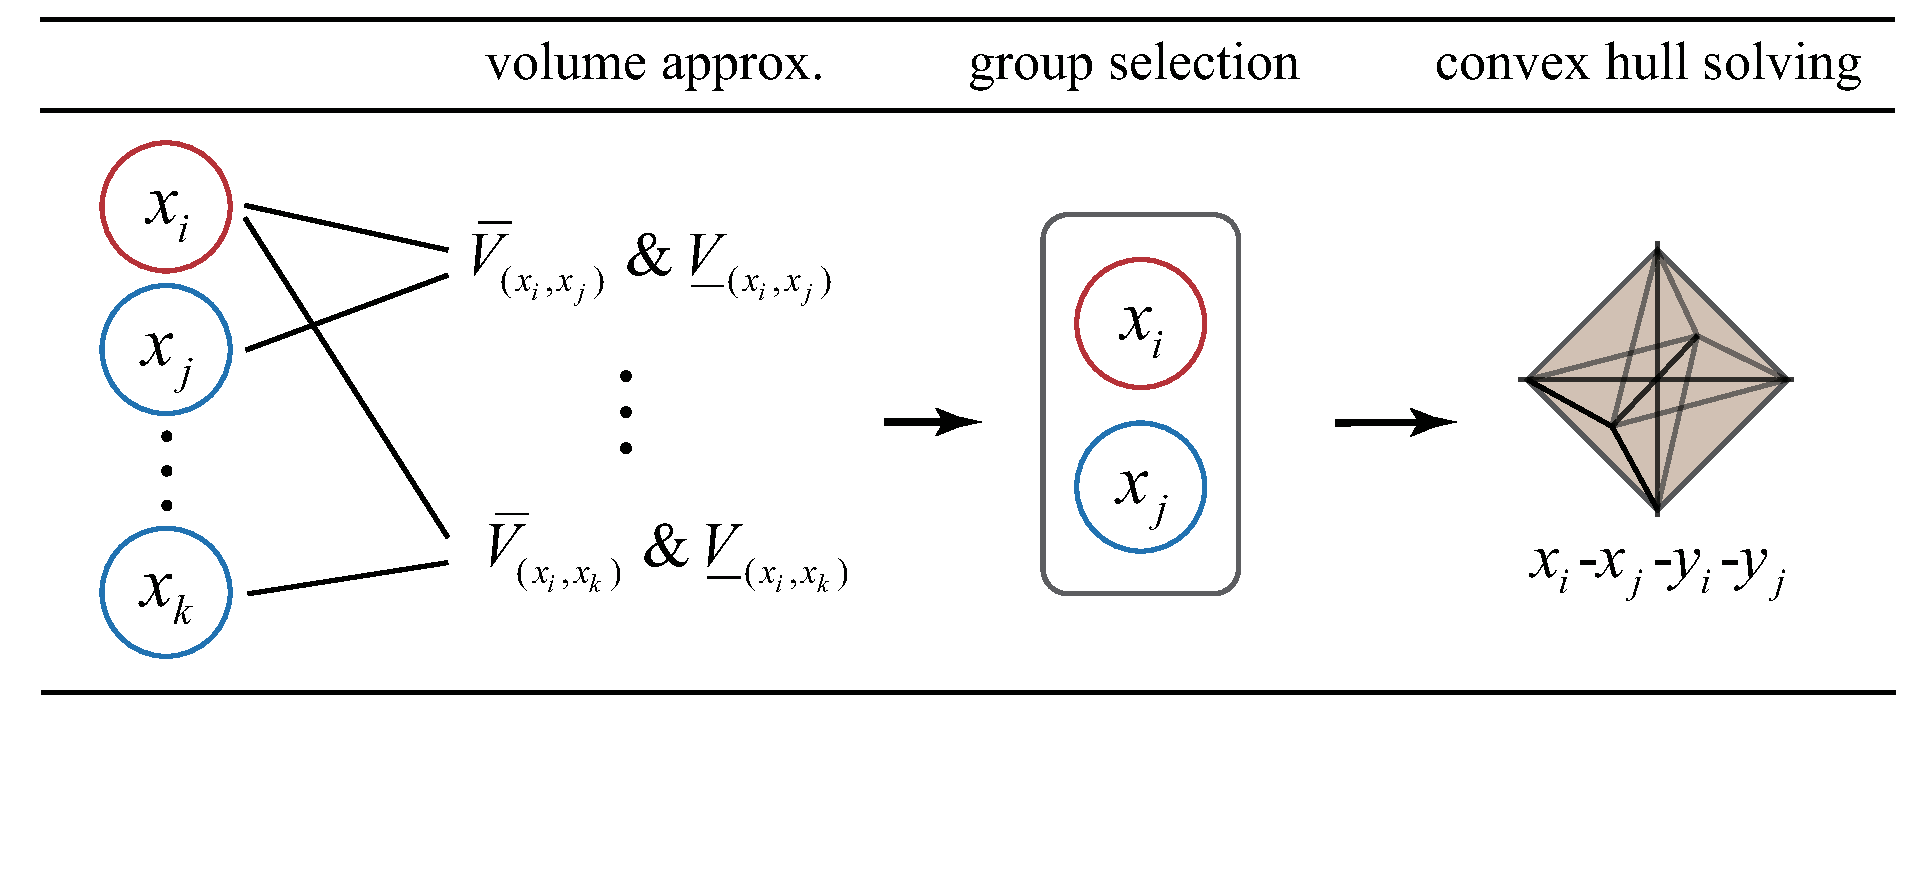
\includegraphics[width=\linewidth]{figures/workflow.eps}
	\caption{Illustration of \ourtool finding a partner neuron for $x_{i}$ and send them
	to compute the four-dimensional convex hull}
	\label{FigR1_0}
	\end{center}
	\vskip -0.2in
\end{figure}\\
\subsubsection{Multi-neuron Relaxation}
The verifiers using $k$-neuron relaxation to compute bounds, like \krelu and \prima, should construct a $k$-dimensional polyhedron $\mathcal{P}$ at first. Then use split, extend, bound, and lift operations, which is called as Split-Bound-Lift Method(SBLM) in \prima, to obtain a $2k$-dimensional polyhedron $\mathcal{C}$ which is regarded as the output constraints in \krelu. $\mathcal{C}$ is well used to bound the outputs from the subsequent activation layers.
\paragraph{Formation of $\mathcal{P}$.}
Generally speaking, any method guaranteeing the input polytope $\mathcal{P}$ is a convex polytope for multi-neuron relaxation is feasible. We give one of the examples in this section, the bound of $x_{i}$ and $x_{j}$ are $[-1,1]$. Next, apply addition and subtraction between these inequalities mutually, an example of doing addition is $\left\{x_{i} + x_{j} \leq \max([-1,1]+[-1,1])=2 \right\}$ , as shown in Figure.~\ref{process_c}(a). Then, add bounds of $x_{i}$ and $x_{j}$ to the constructed constraints, and the input $k$-dimensional polyhedron $\mathcal{P}$ can be generated as the blue part shown in Figure.~\ref{process_c}(b).
%
%
%
\paragraph{Formation of $\mathcal{C}$.} 
Assume that we start with splitting from $x_{i}$ dimension. Specifically, we split polyhedron $\mathcal{P}$ into two parts by halfspaces $\left \{\myvec{x} \in \mathbb{R}^{2} \mid x_{i} \geq 0 \right \}$ and $\left \{\myvec{x} \in \mathbb{R}^{2} \mid x_{i} \leq 0 \right \}$.
The resulting parts are $\left\{ \myvec{x} \in \mathbb{R}^{2} | \myvec{x} \in \mathcal{P} \wedge x_{i} \geq 0 \right\}$
and $\left\{ \myvec{x} \in \mathbb{R}^{2} | \myvec{x} \in \mathcal{P} \wedge x_{i} \leq 0 \right\}$.
Next, we extend these two parts to $(k+1)$ dimension by adding a new dimension $y_{i}$ to $\myvec{x}$. The extension can be regarded as a track of the parallel motion along $y_{i}$ axis by $\mathcal{P}$. The results by extending are presented as $\left\{ \myvec{x} \in \mathbb{R}^{3} | \myvec{x} \in \mathcal{P} \wedge x_{i} \geq 0 \wedge y_{i}\in \mathbb{R} \right\}$ and $\left\{ \myvec{x} \in \mathbb{R}^{3} | \myvec{x} \in \mathcal{P} \wedge x_{i} \leq 0\wedge y_{i}\in \mathbb{R} \right\}$. Note that $\mathcal{P}$  is put into the 3-dimensional space.
\begin{figure*}
\vskip 0.01in 
\begin{center}
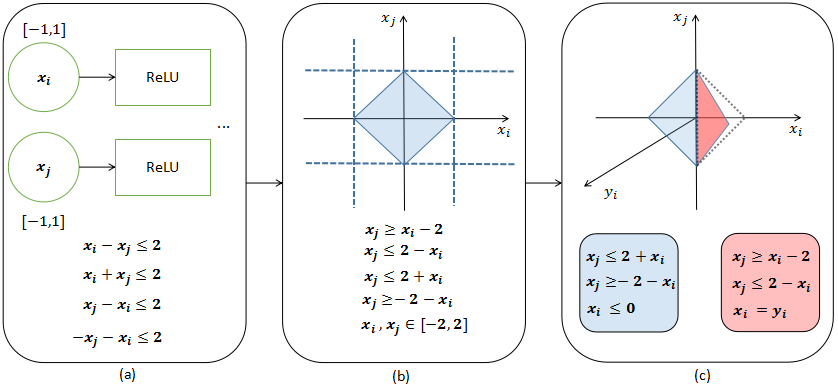
\includegraphics[width=0.85\textwidth]{figures/process_c.png}
\caption{The formation process for $\mathcal{C}_{s}$ and $\mathcal{P}_{s}$ in \relu network.}. \label{process_c}
\end{center}
\vskip -0.01in
\end{figure*}
We then use halfspace depending on activation functions to bound the extensions. For the extension with $\left\{ x_{i} \geq 0 \right\}$, we use halfspace $\left\{ y_{i}=x_{i} \right\}$ to bound it. For the one with $\left\{x_{i} \leq 0 \right\}$, use $\left\{ y_{i} = 0\right\}$ for binding. $\left\{ \myvec{x} \in \mathbb{R}^{3} | \myvec{x} \in \mathcal{P} \wedge x_{i} \geq 0 \wedge y_{i} = x_{i} \right\}$(the red part in Figure.~\ref{process_c}(c))
and $\left\{ \myvec{x} \in \mathbb{R}^{3} | \myvec{x} \in \mathcal{P} \wedge x_{i} \leq 0 \wedge y_{i} = 0 \right\}$(the blue one in Figure.~\ref{process_c}(c)) are the resulting parts.
Finally, we compute the convex hull of the two parts and get a $3$-dimensional convex polyhedron, this step is called a lift. Deal with $x_{j}$ dimension in the same way based on the generated $3$-dimensional polyhedron, then generate a $4$-dimensional polyhedron $\mathcal{C}$. All of the $\mathcal{C}$ from different groups in one layer are taken as an intersection as the constraints for the following layers.

\krelu and \prima directly get $2k$-dimenisonal polyhedra respectively in each split space of $\mathcal{P}_{s}$ through the split, extend, bound, and lift operations, then convex them together to compute $\mathcal{C}_{s}$. Meanwhile, for the convenience of the following proof, the process described above uses split, lift, and bound operations simultaneously for each split space of $\mathcal{P}_{s}$, adding dimension from $k$ to $2k$ step by step. They are equivalent to each other and the proof is given in Theorem.~\ref{theorem2}.

 In \prima, a state-of-the-art depended on \krelu selects groups based on hyperparameters and uses the PDDM method to simplify the constraints, however, the parameters may not always be suitable for different networks and may sacrifice precision. \ourtool aims at automatically selecting some of the groups before computing high-dimensional constraints in PDDM for different networks to save time while maintaining precision. 

%
%
%
\subsubsection{Motivation}
The problem with the classical grouping strategy lies in that it produces
redundant groups for computing the convex hulls, i.e., a multi-neuron relaxation from a group may contain the intersection of the relaxations from other two or more groups. 

Assume that there are three groups: $s_{0}=\left\{x_{i},x_{j} \right\}$, $s_{1}=\left\{x_{i},x_{k} \right\}$ and $s_{2}=\left\{x_{j},x_{k} \right\}$. We observe a situation that the $\mathcal{C}_{0}$ may contain the intersection of the $\mathcal{C}_{1}$ and $\mathcal{C}_{2}$ respectively, then the $s_{0}$ is regarded as the redundant group. For example,  The output constraints $\mathcal{C}_{0} $, $\mathcal{C}_{1}$, and $\mathcal{C}_{2} $ can be expressed as: 

\begin{equation*}
     \begin{aligned}
     &\mathcal{C}_{0}=\left\{x\in \mathbb{R}^{6}\mid \right. \\
                    &-x_{i}+x_{j}-y_{i}-y_{j} \leq 0 \\
                    &x_{i}-x_{j}+y_{i}-y_{j} \leq 2 \\
                    &x_{i}+x_{j}-y_{i}-y_{j} \leq 4\\ 
                    &x_{i}+y_{i}+y_{j} \leq 2\\ 
                    &-x_{i}+x_{j}-y_{j} \leq 4\\ 
                    &x_{i}+x_{j}-y_{j} \leq 0\\ 
                    &y_{j} \leq 1\\ 
                    &y_{i} \leq 1\\ 
                    &x_{i}-y_{i} \leq 1\left.\right\}
	\end{aligned}
     \quad
     \begin{aligned}
     &\mathcal{C}_{1}=\left\{x\in \mathbb{R}^{6}\mid \right. \\
                    &-x_{k}-y_{k} \leq -2 \\
                    &x_{k}+y_{k} \leq 2 \\
                    &x_{i}-y_{i} \leq -1\\ 
                    &x_{i}+y_{i} \leq 1\\                    
                    &x_{i}-x_{k}-y_{k} \leq 0\\ 
                    &-x_{i}+x_{k}+y_{k} \leq 0\\   
                    &x_{i}-y_{i}+y_{k} \leq -2\\
                    &x_{i}-y_{i}-y_{k} \leq 2\\ 
                    &x_{i}+x_{k}+y_{i}+y_{k} \leq 0.5\left.\right\}
	\end{aligned}
     \quad
     \begin{aligned}
     &\mathcal{C}_{2}=\left\{x\in \mathbb{R}^{6}\mid \right. \\
                    &x_{j}-x_{k}-y_{j}-y_{k} \leq 0 \\
                    &x_{j}-x_{k}+y_{j}-y_{k} \leq 2 \\
                    &x_{j}+x_{k}-y_{j}-y_{k} \leq 4\\ 
                    &x_{j}+y_{j}+y_{k} \leq 2\\ 
                    &-x_{j}+x_{k}-y_{k} \leq 4\\ 
                    &x_{j}+x_{k}-y_{k} \leq 0\\ 
                    &y_{k} \leq 1\\ 
                    &y_{j} \leq 1\\ 
                    &x_{j}-y_{j} \leq 1\left.\right\}
	\end{aligned}
\end{equation*}

\iffalse
\begin{equation*}
	\begin{bmatrix}
	-1 & 1 & 0 & -1 & -1 & 0 \\
	1 & -1 & 0 & 1 & 1 & 0 \\
	1 & 1 & 0 & -1 & -1 & 0 \\
	0 & 0 & 0 & 1 & 0 & 0 \\
	-1 & 1 & 0 & 0 & -1 & 0 \\
	1 & 1 & 0 & 0 & -1 & 0 \\
	0 & 0 & 0 & 0 & 1 & 0 \\
	1 & 0 & 0 & 1 & 1 & 0 \\
	1 & 0 & 0 & -1 & 0 & 0
	\end{bmatrix}
	\quad
	\begin{bmatrix}
	0 & 0 & -1 & 0 & 0 & -1 \\
	0 & 0 & 1 & 0 & 0 & 1 \\
	1 & 0 & -1 & 0 & 0 & -1 \\
	-1 & 0 & 1 & 0 & 0 & 1 \\
	1 & 0 & 0 & 1 & 0 & 0 \\
	1 & 0 & 0 & -1 & 0 & 1 \\
	1 & 0 & 0 & 1 & 0 & 0 \\
	1 & 0 & 0 & -1 & 0 & -1 \\
	1 & 0 & 1 & 1 & 0 & 1
	\end{bmatrix}
	\quad
	\begin{bmatrix}
	0 & 1 & -1 & 0 & -1 & -1 \\
	0 & -1 & 1 & 0 & 1 & 1 \\
	0 & 1 & 1 & 0 & -1 & -1 \\
	0 & 0 & 0 & 0 & 0 & 1 \\
	0 & 1 & -1 & 0 & -1 & 0 \\
	0 & 1 & 1 & 0 & -1 & 0 \\
	0 & 0 & 0 & 0 & 1 & 0 \\
	0 & 0 & 1 & 0 & 1 & 1 \\
	0 & 0 & 1 & 0 & 0 & -1
	\end{bmatrix}
\end{equation*}
\fi
where $-1 \leq x_{i},x_{k}\leq 1, -2\leq x_{j}\leq 2$. One can verify that $\mathcal{C}_{0}$ contains the intersection of $\mathcal{C}_{1}$ and $\mathcal{C}_{2}$. We find that for groups containing one neuron $x_{i}$, the redundancy maybe the one with a bigger volume of its $\mathcal{C}$. Additionally, considering the intervals, which can reflect the volume to some extent, maybe a feasible way to select groups, but this may overlook the information in the $\mathcal{P}$ and $\mathcal{C}$.

However, it is unavoidable for high-dimensional calculation for picking out such redundancy precisely, which will spend a lot of time. Because such groups always have a large value of volume, we turn to compute the approximation of volume through the lower dimension to discard redundant groups as much as possible, the groups discarded are also called worse groups in the following.

\ourtool can efficiently identify the worse groups before solving the convex hull problems.
As a result, it produces neuron groups that have fewer redundant groups while considering the multi-neuron relaxation to preserve precision.


%
%
%
\subsubsection{\ourtool Algorithm}
The key idea behind \ourtool is \emph{fast computing the volume approximations of all possible
$k$-neuron groups.}
If the volume approximation for the group $\left\{x_{i},x_{j}\right\}$ is smaller than the ones for 
any other groups', such as $\left\{x_{i},x_{k}\right\}$,
then we choose $\left\{x_{i},x_{j}\right\}$ as the selected group. 
Figure.~\ref{FigR1_0} shows the workflow of \ourtool finding a partner for neuron $x_{i}$.
It has the following three steps:

\paragraph{Volume approximation.}
Computing the precise volume of a $(2k)$-dimensional convex hull
formed by a $k$-neuron group can be time-consuming (i.e., the volume of the convex hull
$x_{i}\text{-}x_{j}\text{-}y_{i}\text{-}y_{j}$ in Figure.~\ref{FigR1_0}). Therefore,
we compute the approximation method in Section~\ref{mvee} to under and over-approximate the volumes
of convex hulls for each group, in order to select groups which will be computed a $(2k)$-dimensional convex hull. The volume approximation method used in \ourtool is based on Betke et al.~\cite{betke1993approximating}, and we improve the over-approximation by using the volume of $\mathcal{P}$ to make the approximation tighter. Our approximation is computed on $k$-dimension(particularly in computation for the volume of $\mathcal{P}$ by existing volume tools) and is used to reduce some of the $(2k)$-dimensional computations.
%For instance, both of the bound for $x_{i}$ and $x_{j}$ from $\mathcal{P}$ are $[-1,1]$ and the $k$-dimensional volume of $\mathcal{P}$ is $1$. Then, the over-approximation for volume of $\mathcal{C}$ is $(1-0)^{2}\times1 = 1$, and the under one is $(1/24)\times(1-(-1))^{2}\times(1-0)^{2} = 1/6$, according to our approximation method. 

\paragraph{Neurons grouping selection.}
Once all under and over-approximated volumes have been computed for the groups,
select the groups for each neuron, like $x_{i}$, whose over-approximation volumes are smaller than most of the under-approximation volumes of other groups.
\iffalse
For instance, there are totally three groups containing $x_{i}$ in one layer: $\left\{ x_{i},x_{j} \right\}$, $\left\{ x_{i},x_{k} \right\}$, and $\left\{ x_{i},x_{h} \right\}$. The approximations of these groups can be presented as intervals respectively: $[2,1]$, $[1.5,0.5]$, and $[0.7,0.4]$.
At first, we remain an empty set $\mathcal{G}_{i}$ for selected groups and traversal to $\left\{x_{i},x_{j} \right\}$. When the $\mathcal{G}_{i}$ is empty so we directly add $\left\{x_{i},x_{j} \right\}$ to $\mathcal{G}_{i}$. Then we traversal to $\left\{x_{i},x_{k} \right\}$, its interval has overlap with the union of the intervals in $\mathcal{G}_{i}$, we record $\left\{x_{i},x_{k} \right\}$ in $\mathcal{G}_{i}$. However, the over-approximation of $\left\{ x_{i},x_{h}\right\}$ equals 0.7 is less than the maximal under-approximations among groups in $\mathcal{G}$(which is 0.7). In this situation, we replace all groups in current $\mathcal{G}_{i}$ with $\left\{ x_{i},x_{h}\right\}$. If the interval from $\left\{ x_{i}, x_{h}\right\}$ is $[2.1,1.6]$ of which under-approximation is more than the minimal over-approximations among groups in $\mathcal{G}_{i}$(which is 1.5), $\left\{ x_{i},x_{h}\right\}$ will not be added to $\mathcal{G}_{i}$. \\%The process is described in Figure.~ .
\fi
Our strategy prefers selecting the groups which avoid the phenomenon in our motivation while maintaining groups as many as possible to guarantee precision and saving time as possibly as possible. More details can be found in Section~\ref{Subsec3.4}.
%When finding partner for another input, its volume with $x_{i}$
%is already available.

\paragraph{Convex hull solving.}
Once the groups of each neuron are determined, they are sent to derive their exact $(2k)$-dimensional convex hull,
like $\left\{x_{i},x_{j}\right\}$ in Figure.~\ref{FigR1_0}.
We use the solver in \prima~\cite{DBLP:journals/pacmpl/MullerMSPV22} to accomplish this task.
It provides worst-case time-complexity convex hull computation
and guarantees exactness, making it a suitable choice
for our work.
Using the intersection of these computed convex hulls, the bounds of $y_{i}$ and $y_{j}$
can be obtained by a linear programming(LP) solver.
With these bounds for the neurons in a layer, \ourtool can then determine the groups for the subsequent layer.\\
In Section~\ref{sec:pre}, we introduce the formation process for multi-neuron convex relaxation, which is used in Section~\ref{mvee}, where we present formulas for under and over-approximation.

%
%
%

\section{Preliminaries}
\label{sec:pre}
This section reviews some notions needed for understanding our approach.


\subsection{Neural Network Verification}
A \emph{(feedforward) neural network} $\myvec{h}(\myvec{x}): \mathcal{X} \to
\mathbb{R}^{|\mathcal{Y}|}$ is a $|\mathcal{Y}|$-dimensional vector
valued function from the input space $\mathcal{X}$ to the output space
$\mathcal{Y}$.  Specifically, $\myvec{h}(\myvec{x})$ is the
interleaved composition of affine function layers
$\myvec{g}_i(\myvec{x})=\mymatrix{W}_i\myvec{x}+\myvec{b}_i$, with
non-linear activation layers $\myvec{f}_i(\myvec{x})$:
\[
\myvec{h}(\myvec{x}) = \myvec{g}_{L} \comp \myvec{f}_{L} \comp
\myvec{g}_{L-1} \comp \cdots \comp \myvec{f}_{1} \comp
\myvec{g}_{0}(\myvec{x})
\]
where $L$ is the number of hidden layers. 
$\myvec{f}_i(\myvec{x})$ applies non-linear activation functions in an element-wise manner. 
If $\myvec{h}(\myvec{x})$ is a classification neural network, it will
output the index $c$ of its maximum output vector component, i.e. $c =
\arg \max_{j} \myvec{h}(\myvec{x})_{j}$.

Neural network verification problem commonly needs to verify the
\emph{robustness} property.  A robust neural network must satisfy the
smoothness assumption~\cite{DBLP:books/daglib/0040158}, i.e., for any
input $\myvec{x}$ and a small perturbation $\myvec{\delta}$,
$\myvec{h}(\myvec{x} + \myvec{\delta}) \approx \myvec{h}(\myvec{x})$ should
 hold. In the case of classification tasks, this assumption conforms
to the visual capabilities of human: if $\myvec{x}$ looks similar to
$\myvec{x}'$, they should belong to the same class.

Formally, perturbed inputs are defined by a $p$-norm ball neighborhood
of $\myvec{x}$:
\[
\mathbb{B}^{p}_{\varepsilon} = \{\myvec{x}' = \myvec{x}
+ \myvec{\delta} \mid \|\myvec{\delta}\|_{p} \leq \varepsilon\}
\]
where $\varepsilon$ is the \emph{perturbation threshold} that bounds
$\myvec{\delta}$. We would like to verify that the neural network
$\myvec{h}(\myvec{x})$ does not misclassify any perturbed input in
this region.

\begin{definition}
Given a neural network $\myvec{h}(\myvec{x})$, an input
$\myvec{x}\in\mathcal{X}$ and a perturbation threshold $\varepsilon$, a
\emph{verification problem} is to give the true value of the
following statement:
\begin{equation}
\begin{aligned}
  &\arg \max_{j} \myvec{h}(\myvec{x})_{j} = \arg \max_{j}
  \myvec{h}(\myvec{x}')_{j},\\
 &\mbox{ for each } \myvec{x}' \in
  \mathbb{B}^{p}_{\varepsilon}(\myvec{x}).\nonumber
\end{aligned}
\end{equation}
\end{definition}

If the above statement is true, then we can conclude that the neural network
$\myvec{h}$ is robust with respect to the input $\myvec{x}$ against
the perturbation threshold $\varepsilon$.

%
%
%

\subsection{Formation for multi-neuron relaxation}\label{Subsec3.2}

The formation from \krelu is utilized in both of \prima and \ourtool to generate output constraints $\mathcal{C}_{s}$.
Formally, for a $k$-dimensional input polytope $\mathcal{P}_{s}=\left \{\myvec{x} \in \mathbb{R}^{k}\mid \mymatrix{A}\myvec{x}\leq \myvec{b}\right\}$ generated by a set of $k$ neurons $s\subseteq \mathcal{S}$, $\mathcal{S}$ is the set of all neurons,
 the input polytope $\mathcal{P}_{s}$ will generate a higher-dimensional polyhedron $\mathcal{C}_{s} \subseteq \mathbb{R}^{2k}$.
In this section, we introduce the formation and definition for $\mathcal{C}_{s}$.

The input polytope $\mathcal{P}_{s}$ can be constructed by any method which uses the relaxation among neurons in group $s$ to guarantee $\mathcal{P}_{s}$ is a convex polytope, with linear inequations for the  convenience of LP solver, like the process in \prima.  
%\subsection{Formation of input polyhedron $\mathcal{P}_{s}$}\label{form_P}
%In the $p$-th layer with $n_{p}$ neurons, these neurons can be expressed by the neurons in the previous layer, which can be defined as a set of constraints $\left\{ \mymatrix{A}_{i}\myvec{x}^{(p-1)} \leq \myvec{1}x_{i}^{(p)}, \mymatrix{A}_{i}\myvec{x}^{(p-1)} \geq \myvec{1}x_{i}^{(p)} \right\}, \forall I \in \llbracket n_{p} \rrbracket $, where $\myvec{1}$ is a unit vector. Then, for each grouping, add or subtract the constraints of neurons pairwise, and a $k$-dimensional polyhedron $\mathcal{P}$ is generated. At the last, add the lower and upper bound from once symbolic interval propagation of each neuron to the polyhedron, and the $\mathcal{P}_{s}$ is completed. 

\subsubsection{Formation of multi-neuron relaxation $\mathcal{C}_{s}$}
Among the formation of $\mathcal{C}_{s}$, we have four main steps: split, extend, bound, and lift.
We start by splitting space from $x_{i}$ dimension. Specifically, we split $\mathcal{P}_{s}$ into two parts with halfspaces $t_{i}^{+}=\left \{\myvec{x} \in \mathbb{R}^{k} \mid x_{i} \geq c \right \}$ and $t_{i}^{-}=\left \{\myvec{x} \in \mathbb{R}^{k} \mid x_{i} \leq c \right \}$(start from $\forall x_{i} \in s$ is valid, and c is a constant~\cite{DBLP:journals/pacmpl/MullerMSPV22}).
The resulting parts are $\mathcal{P}_{s} \cap t_{i}^{\left\{+,-\right\}}$ respectively. 
Next, we extend $\mathcal{P}_{s} \cap t_{i}^{\left\{+,-\right\}}\subseteq \mathbb{R}^{k}$ to $(k+1)$ dimension by adding a new dimension to $\myvec{x}$, marked as $y_{i}$, and defining the extension as $e(\mathcal{P}^{(i)}_{s} \cap t_{i}^{\left\{+,-\right\}})\subseteq \mathbb{R}^{k+1}$. 
Then we use halfspaces $\mathcal{B}_{i}^{\left\{+,-\right\}} = \left\{ \myvec{x} \in \mathbb{R}^{k+1} | y_{i}=u^{\left\{+,-\right\}}_{i}(x_{i})\cup y_{i}=l^{\left\{+,-\right\}}_{i}(x_{i}),\forall \myvec{x} \in e(\mathcal{P}^{(i)}_{s} \cap t_{i}^{\left\{+,-\right\}})\right\}$ to bound the extensions. For \relu, $u^{\left\{+,-\right\}}_{i}(\cdot)=l^{\left\{+,-\right\}}_{i}(\cdot)$. The resulting parts are defined as $e(\mathcal{P}^{(i)}_{s} \cap t_{i}^{+} ) \cap \mathcal{B}_{i}^{+}$ and $e(\mathcal{P}^{(i)}_{s} \cap t_{i}^{-} ) \cap \mathcal{B}_{i}^{-}$, when the activation function is $f(\cdot)$, $u^{\left\{+,- \right\}}_{i}(\cdot)$ and $l^{\left\{+,- \right\}}_{i}(\cdot)$ are four linear functions satisfying $l^{\left\{+,- \right\}}_{i}(x_{i}) \leq f(x_{i}) \leq u^{\left\{+,- \right\}}_{i}(x_{i}), \forall x_{i} \in e(\mathcal{P}^{(i)}_{s} \cap t_{i}^{\left\{+,-\right\}})$. 
Finally, compute the convex hull of the two parts and get a $(k+1)$-dimensional convex polyhedron, which is the lift step. Deal with other dimensions in $\mathcal{P}_{s}$ in the same way until generating a $(2k)$-dimensional polyhedron $\mathcal{C}_{s}$, shown by Definition.~\ref{Def3}.


\begin{definition}\label{Def3}
For $k$ selected inputs $x_{0},x_{1},...,x_{k-1}$, their multi-neuron relaxation formed from Section~\ref{Subsec3.2} is defined as
$\mathcal{C}_{s}$ where $s = \left \{x_{0},x_{1},...,x_{k-1}\right \}$. 
$conv(\cdot)$ implies the convex hull for the set of points. 
There has an equation according to the process in Section~\ref{Subsec3.2}:
\begin{equation}\label{C}
\begin{aligned}
\mathcal{P}_{s}^{(i+1)} &= conv( e(\mathcal{P}^{(i)}_{s} \cap t_{i}^{+} ) \cap \mathcal{B}_{i}^{+}\\ 
&\cup e(\mathcal{P}^{(i)}_{s} \cap t_{i}^{-} ) \cap \mathcal{B}_{i}^{-}), \forall i \in \llbracket  k \rrbracket
\end{aligned}
\end{equation}
where:
\begin{equation*}
\begin{aligned}
&\mathcal{P}_{s}^{(0)} = \left\{ \myvec{x} \in \mathbb{R}^{k}|\myvec{x} \in \mathcal{P}_{s} \right\};\mathcal{P}_{s}^{k}=\mathcal{C}_{s}\\
&t_{i}^{+} = \left\{ \myvec{x} \in \mathbb{R}^{k+i}|x_{i} \geq c \right\};t_{i}^{-} = \left\{ \myvec{x} \in \mathbb{R}^{k+i}|x_{i} \leq c \right\}\\
&\mathcal{B}_{i}^{\left\{+,-\right\}} = \left\{ \myvec{x} \in \mathbb{R}^{k+1} | y_{i}=u^{\left\{+,-\right\}}_{i}(x_{i}),y_{i}=l^{\left\{+,-\right\}}_{i}(x_{i}),\forall \myvec{x} \in e(\mathcal{P}^{(i)}_{s} \cap t_{i}^{\left\{+,-\right\}}) \right\} \\
&e(\mathcal{D}):\mathbb{R}^{i} \leftarrow \mathbb{R}^{i}\times \mathbb{R}, \mathcal{D} = \left\{ \myvec{x}|\myvec{x}\in \mathbb{R}^{i} \right\}
\end{aligned}
\end{equation*}
$t_{i}^{\left\{+,- \right\}}$ means the split space, $\mathcal{B}_{i}^{\left\{+,- \right\}}$ is the added bounds according to $t_{i}^{\left\{+,- \right\}}$, $e(\mathcal{D})$ is the function for adding a dimension to the  set of points $\mathcal{D}$, $u^{\left\{+,-\right\}}_{i}(\cdot)$ and $l^{\left\{+,-\right\}}_{i}(\cdot)$ satisfy $l^{\left\{+,- \right\}}_{i}(x_{i}) \leq f(x_{i}) \leq u^{\left\{+,- \right\}}_{i}(x_{i}), \forall x_{i} \in e(\mathcal{P}^{(i)}_{s} \cap t_{i}^{\left\{+,-\right\}})$. The definition is equal to the description from \prima and the proof can be found in Theorem.~\ref{theorem2}.
\end{definition}

%
%
%

\section{Volume Approximation Based Grouping}\label{Sec3}
\label{sec:method}

In this section, we provide our improved neurons grouping
strategy for $k$-neuron($k \in Z^{+}, k \geq 2$) convex relaxation.
Assume that we are dealing with $n_{p}$ neurons in the $p$-th layer of a fully connected layer, these $n_{p}$ value of neurons marked as $x_{0},x_{1},...,x_{n_{p}-1}$, and a set $\mathcal{S}=\left \{x_{0},x_{1},...,x_{n_{p}-1}\right \}$.
The formalization and soundness proof for \ourtool will be provided in the following.

%
%
%
\subsection{Volumes Approximation of \ourtool}\label{mvee}
In this section, we focus on how to approximate to guide the neuron grouping in multi-neuron convex relaxation methods while maintaining its soundness. This can reduce the $2k$-dimensional calculation to a $k$-dimensional one. 

\subsubsection{Under-approximation}\label{mvee}

The most time-consuming procedure step in multi-neuron relaxation is the 
computation of convex hull , which is an NP-hard problem as in traditional methods.
Rather than computing the convex hull for each $k$-neuron group
in traditional ways,
we compute a volume approximation of them.
The volume approximation is then used to guide grouping.

For a convex polyhedron $\mathcal{K} \in \mathbb{R}^{d}$, its
over and under-approximations of volume, denoted as $\overline{V}(\mathcal{K})$ and $\underline{V}(\mathcal{K})$ respectively,
have the following relation~\cite{elekes1986geometric}:
$$
\frac{\overline{V}(\mathcal{K})}{\underline{V}(\mathcal{K})} \geq \left(\frac{cd}{\log d}\right)^{d}
$$\\
where exists a constant $c$.
One such algorithm from Betke et al.
can obtain $\overline{V}(\mathcal{K}) = \prod_{i=0}^{d-1}(u_{i}-l_{i})$ and $\underline{V}(\mathcal{K}) = \prod_{i=0}^{d-1}(u_{i}-l_{i})/d!$, $[l_{i},u_{i}]$ implies the range of the i-th dimension in $\mathcal{K}$.
We use $\underline{V}(\mathcal{K})$ as under-approximation in \ourtool, and generate tighter approximation based on
the idea presented by Betke et al. to guide well for grouping strategy while keeping soundness. 
%
%
%
\subsubsection{Over-approximation}
We present the formulas of the under and over-approximation used in \ourtool and provide the proof about the over-one based on the definition in Section.~\ref{Subsec3.2}.
\begin{theorem}
\label{theorem1}
(Approximation formation). $VoL(\mathcal{C}_{s})$ can be bounded by $\overline{V}_{s}$ and $\underline{V}_{s}$ as follows:

\begin{equation}\label{over}
\overline{V}_{s} = VoL(\mathcal{P}_{s}) \cdot \prod_{i\in \llbracket  k \rrbracket}^{}(\overline{f}_{i} - \underline{f}_{i})
\end{equation}

\begin{equation}\label{under}
\underline{V}_{s} = \dfrac{1}{(2k)!} \cdot \prod_{i\in \llbracket  k \rrbracket}^{} (u_{i} - l_{i}) \cdot(\overline{f}_{i} - \underline{f}_{i})
\end{equation}
where $\overline{f}_{i} = \max(u^{+ }_{i}(x_{i}),u^{-}_{i}(x_{i}))$, $\underline{f}_{i} = \min(l^{+ }_{i}(x_{i}),l^{-}_{i}(x_{i}))$, $\forall x_{i} \in  e(\mathcal{P}^{(i)}_{s} \cap t_{i}^{\left\{ +, -\right\}} )$.
%Here, $y_{i}=f(x_{i})$ and for each $i\in \{1,\ldots,k\}$, $\underline{f}_{i} \leq y_{i} \leq \overline{f}_{i}$ where $x_{i} \in s$. 
%$i \in \llbracket   n  \rrbracket$.
\end{theorem}

\begin{proof} 
%The under-approximation is generated from the Theorem.2 directly in Betke et al.~\cite{betke1993approximating}. However, 
The structure of $\mathcal{C}_{s}$ is unique, allowing us to derive a tighter over-approximation than the one described in Betke et al.\\
Regarding the over-approximation, we have the following: 

\begin{equation*}
\begin{aligned}
\because &\mathcal{B}_{i}^{+} \subseteq \left\{\myvec{x}\in \mathbb{R}^{k+i+1}|y_{i}\leq \overline{f}_{i}, x_{i}\in e(\mathcal{P}^{(i)}_{s} \cap t_{i}^{+}) \right\};\\
& \mathcal{B}_{i}^{-} \subseteq \left\{\myvec{x}\in \mathbb{R}^{k+i+1}|y_{i}\geq \underline{f}_{i}, x_{i}\in e(\mathcal{P}^{(i)}_{s} \cap t_{i}^{-}) \right\};\\
& \mathcal{P}_{s}^{(i+1)} = conv( e(\mathcal{P}^{(i)}_{s} \cap t_{i}^{+} ) \cap \mathcal{B}_{i}^{+}
\cup e(\mathcal{P}^{(i)}_{s} \cap t_{i}^{-} ) \cap \mathcal{B}_{i}^{-}), \forall i \in \llbracket  k \rrbracket \\
\therefore  &P_{s}^{(i+1)} \subseteq conv( e(P^{(i)}_{s} ) \cap \left\{\myvec{x}\in \mathbb{R}^{k+i+1}|y_{i}\leq \overline{f}_{i} \right\}\\
 &\cup e(P^{(i)}_{s} ) \cap \left\{\myvec{x}\in \mathbb{R}^{k+i+1}|y_{i}\geq \underline{f}_{i} \right\}, \forall i \in \llbracket  k \rrbracket)
\end{aligned}
\end{equation*}

The right-hand side of the above equation can be regarded as the extension of $\mathcal{P}_{s}^{(i)}$ along the $y_{i}$ axis. The extension is intersected by the planes $y_{i} = \overline{f}_{i}$ and $y_{i}=\underline{f}_{i}$, and the content of the intersected extension is the over-approximation for $\mathcal{P}_{s}^{(i+1)}$. Based on the definition of a prism~\cite{sommerville2020introduction}, a $k$-dimensional prism is formed by the parallel motion of a $(k-1)$-dimensional polytope, the base content $S$ of the prism is the volume of the $(k-1)$-dimensional polytope and its height $h$ equals to the distance of the parallel motion.
Because the $\mathcal{P}_{s}^{i}$ corresponds to the $(k-1)$-dimensional polytope, and the extension of $\mathcal{P}_{s}^{i}$ along the $y_{i}$ axis, which is cutten by planes $y_{i} = \overline{f}_{i}$ and $y_{i} = \underline{f}_{i}$, corresponds the distance of parallel motion between planes $y_{i} = \overline{f}_{i}$ and $y_{i} = \underline{f}_{i}$. Therefore, the over-approximation of $VoL(P^{(i+1)}_{s})$ is a volume of prism with a base content of $VoL(\mathcal{P}_{s}^{(i)})$ and a height of $\overline{f}_{i} - \underline{f}_{i}$. 
 

\begin{equation*}
\begin{aligned}
&\therefore VoL(P^{(i+1)}_{s}) \leq VoL(P^{(i)}_{s}) \cdot (\overline{f}_{i}-\underline{f}_{i})\\
&\therefore VoL(\mathcal{C}_{s}) \leq VoL(\mathcal{P}_{s}) \cdot \prod_{i\in \llbracket  k \rrbracket}^{}(\overline{f}_{i} - \underline{f}_{i})
\end{aligned}
\end{equation*}
\\
Because $VoL(\mathcal{P}_{s})$ is $k$-dimensional, it is easier to compute an actual value which is also over-approximated in Betke et al., so $\overline{V}_{s}$ in \ourtool is tighter.

\end{proof}

%
%
%

\subsection{Detailed algorithm of \ourtool}\label{Subsec3.4}

We now present the detailed 
workflow of \ourtool in Algorithm ~\ref{algorithm1}.
It takes as input a set $\mathcal{S}$ that needs to be grouped,
the pre-computed lower bounds $\mathcal{L}$ and upper bounds $\mathcal{U}$ of these neurons, and
outputs the group $\mathcal{G}$ which will be sent to PDDM, the instrument in \prima.

\begin{algorithm}[!h]
   \caption{\ourtool Grouping Strategy for a Layer}
   \label{algorithm1} 
\begin{algorithmic}[1]
   \STATE {\bfseries Input:} Input set $\mathcal{S}$ need to be grouped of the layer,
 pre-computed bounds $\mathcal{L}$ and $\mathcal{U}$ of the layer.


   \STATE  $\mathcal{G} \leftarrow \emptyset$
   \FOR{$x_{i}$ in $\mathcal{S}$}
	\FOR{$s$ \text{containing} $x_{i}$ \text{in} $\mathcal{S}$}

   \IF{$\overline{V}_{s} = \varnothing$ }
	
   \STATE Create region: $\mathcal{P}_{s}$ $\leftarrow$ GET\_REGION(s, $\mathcal{L}, \mathcal{U}$)
   %\STATE Turn to vertex-representation: v $\leftarrow$ con2ver(h)
   \STATE Volume approxiamtion: $\overline{V}_{s} \leftarrow$ Equation~\ref{over}, $\underline{V}_{s} \leftarrow$ Equation~\ref{under}
   \STATE Updating $\mathcal{G}_{i}$: $\mathcal{G}_{i} \leftarrow$ UPDATE($\mathcal{G}_{i}$,$\overline{V}_{s}$, $\underline{V}_{s}$)  

   \ENDIF

   
   \IF{$\mathcal{G}_{i}$}
	
   \STATE Add to final group: $\mathcal{G} = \mathcal{G} \cup \mathcal{G}_{i}$

   \ENDIF

   \ENDFOR
   \ENDFOR
   \STATE Return $\mathcal{G}$
\end{algorithmic}
\end{algorithm}
%, and consider several groups whose reachable sets of $VoL(\mathcal{C}_{s})$ overlap with each other as $\mathcal{G}_{i}$(line 8). Formally, $\forall s_{1}, s_{2} \in \mathcal{G}_{i}$, it must hold that $max(\underline{V}_{s_{1}},\underline{V}_{s_{2}}) \leq min(\overline{V}_{s_{1}},\overline{V}_{s_{2}})$.
For $x_{i}$, \ourtool collects all groups containing $x_{i}$ (lines 2 to 4).
Line 6 calculates the halfspace-representation of $\mathcal{P}_{s}$~\cite{gaubert2011minimal}. 
Once the volume approximations of all possible groups for $x_{i}$ are calculated(line 7),
\ourtool chooses the groups that have smaller over-approximations as $\mathcal{G}_{i}$ by Algorithm~\ref{algorithm2}(line 8),
the $VoL(\mathcal{P}_{s})$ with low dimension can be easily computed by Qhull~\cite{barber2013qhull}. 

Specifically, we compute all the volume $\overline{V}_{s}$ and $\underline{V}_{s}$ for $s$ containing $x_{i}$ using equation~\ref{over} and~\ref{under}.
Traverse $\overline{V}_{s}$ and $\underline{V}_{s}$ for all $s \subseteq \mathcal{S}$, 
if there is a group $s \notin \mathcal{G}_{i}$ that satisfies $\overline{V}_{s} \leq \max_{j\in \mathcal{G}_{i}}(\underline{V}_{j})$, let $\mathcal{G}_{i} = \left \{s\right \}$. If $\underline{V}_{s} \geq \min_{j\in \mathcal{G}_{i}}(\overline{V}_{j})$, ignore this $s$, otherwise, add $s$ to set $\mathcal{G}_{i}$. After that, continue to traverse $\overline{V}_{s}$ and $\underline{V}_{s}$ to make the set $\mathcal{G}_{i}$ as the set of groups selected for neuron $i$.
Finally, adds $\mathcal{G}_{i}$ to $\mathcal{G}$ or do nothing if no group is found(line 10 to 11).
\begin{algorithm}[!h]
   \caption{a strategy for selecting groups UPDATE}
   \label{algorithm2} 
\begin{algorithmic}[1]
   
   \STATE {\bfseries Input:} group set $\mathcal{G}_{i}$ and the approximations $\overline{V}_{s}$ and $\underline{V}_{s}$.
   

   \IF{$\mathcal{G}_{i}= \emptyset$}
   \STATE $\mathcal{G}_{i}= \left\{s \right\}$
   \ELSIF {$\overline{V}_{s} \leq \max_{j\in \mathcal{G}_{i}}(\underline{V}_{j})$}
   \STATE $\mathcal{G}_{i} = \left \{s\right \}$
   \ELSIF {$\underline{V}_{s} \geq \min_{j\in \mathcal{G}_{i}}(\overline{V}_{j})$}
   \STATE pass
   \ELSE
   \STATE Add $s$ to $\mathcal{G}_{i}$
   \ENDIF
   \STATE Return $\mathcal{G}_{i}$

\end{algorithmic}
\end{algorithm}

The resulting set $\mathcal{G}$ for a layer is then passed to the PDDM~\cite{DBLP:journals/pacmpl/MullerMSPV22} to obtain their $(2k)$-dimensional convex hulls. 
From the intersection of these convex hulls, $\mathcal{L}$ and $\mathcal{U}$ for each neuron member's lower and upper bounds in the next layer, respectively, can be obtained using an LP solver.
Then Algorithm~\ref{algorithm1} can be recursively applied to find groups for the next layer. 
%
%
%
\subsection{Equivalency proof}\label{equivalency proof}
Before proving our description of $\mathcal{C}$ equals to the one in \prima. We give the description of $\mathcal{C}$ in \prima, using the symbols in Definition.~\ref{Def3} through convexity preserving~\cite{li1999convexity}:
\begin{equation}\label{prima C}
\mathcal{C}_{s} = conv\big( \bigcup_{t} ( e^{k}(\mathcal{P}_{s}^{(0)})\cap \bigcap_{i \in s}^{}t_{i}^{\left\{ +,-\right\}} \cap \bigcap_{i \in s}^{}\mathcal{B}_{i}^{\left\{ +,-\right\}} ) \big)
\end{equation}
where $t$ means any combination of $t_{i}^{\left\{ + \right\}}$ or $t_{i}^{\left\{ - \right\}}$, $\forall i \in s$, $e^{k}(\cdot)$ means do $k$ times extend operations on the set. 
\begin{theorem}
\label{theorem2}
(Equivalency proof). The Definition.~\ref{Def3} is equivalent to Equation.~\ref{prima C}.
\begin{proof}
Use the convexity preserving and the definition of the $e(\cdot)$, $t/ t_{i}^{\left\{+,- \right\}}$ means the combinations without $t_{i}^{\left\{+,- \right\}}$, we can get following equations:

\begin{equation*}
\begin{aligned}
&\mathcal{C}_{s} =  conv\big( e^{k}( \mathcal{P}_{s}^{(0)})\cap   \bigcup_{t} (\bigcap_{i \in s}^{}t_{i}^{\left\{ +,-\right\}} \cap \bigcap_{i \in s}^{}\mathcal{B}_{i}^{\left\{ +,-\right\}})\big)\\
%
&= conv\big( (e^{k}( \mathcal{P}_{s}^{(0)})\cap  \bigcup_{t/t^{-}_{0}} (t_{0}^{+} \cap \mathcal{B}_{0}^{+} \cap \bigcap_{i \in s/0}^{}t_{i}^{\left\{ +,-\right\}} \cap \bigcap_{i \in s/0}^{}\mathcal{B}_{i}^{\left\{ +,-\right\}}))\\
& \cup (e^{k}( \mathcal{P}_{s}^{(0)})\cap \bigcup_{t/t^{+}_{0}} (t_{0}^{-} \cap \mathcal{B}_{0}^{-} \cap \bigcap_{i \in s/0}^{}t_{i}^{\left\{ +,-\right\}} \cap \bigcap_{i \in s/0}^{}\mathcal{B}_{i}^{\left\{ +,-\right\}})) \big)\\
%
&= conv\big( e^{k-1}( e(\mathcal{P}_{s}^{(0)})\cap( t_{0}^{+}\cap \mathcal{B}^{+}_{0} \cup t_{0}^{-}\cap \mathcal{B}^{-}_{0}))\cap \!\!\!\!  \bigcup_{t/t_{0}^{\left\{+,- \right\}}}\!\! (\bigcap_{i \in s/0}^{}t_{i}^{\left\{ +,-\right\}} \cap\!\! \bigcap_{i \in s/0}^{}\!\! \mathcal{B}_{i}^{\left\{ +,-\right\}})\big)\\
%&= conv\big( e^{k-1}( e(\mathcal{P}_{s}^{(0)})\cap t_{0}^{+}\cap \mathcal{B}^{+}_{0} )\cap   \bigcup_{t} (\bigcap_{i \in s/0}^{}t_{i}^{\left\{ +,-\right\}} \cap \bigcap_{i \in s/0}^{}\mathcal{B}_{i}^{\left\{ +,-\right\}}) \\
%&\cup e^{k-1}( e(\mathcal{P}_{s}^{(0)})\cap t_{0}^{-}\cap \mathcal{B}^{-}_{0} )\cap \bigcup_{t} (\bigcap_{i \in s/0}^{}t_{i}^{\left\{ +,-\right\}} \cap \bigcap_{i \in s/0}^{}\mathcal{B}_{i}^{\left\{ +,-\right\}})\big)\\
&= conv\big(e^{k-1}(\mathcal{P}_{s}^{(1)}) \cap   \bigcup_{t/t_{0}^{\left\{ +,-\right\}}} (\bigcap_{i \in s/0}^{}t_{i}^{\left\{ +,-\right\}} \cap \bigcap_{i \in s/0}^{}\mathcal{B}_{i}^{\left\{ +,-\right\}} \big)\\
&= ...\\
&= conv\big( e(\mathcal{P}^{(k-1)}_{s} \cap t_{k-1}^{+} ) \cap \mathcal{B}_{k-1}^{+}\cup e(\mathcal{P}^{(k-1)}_{s} \cap t_{k-1}^{-} ) \cap \mathcal{B}_{k-1}^{-}\big) = \mathcal{P}_{s}^{(k)}
\end{aligned}
\end{equation*}
The left of the equation is equivalent to the right, so the theorem is proven. 
\end{proof}
\end{theorem}
%
%
%
\subsection{Generalizaion}\label{sec-generalization}
\ourtool supports fast grouping with common activation functions.
According to Algorithm~\ref{algorithm1},
\ourtool avoids $2k$-dimensional calculation
by approximating volume with a $k$-dimensional polyhedron $\mathcal{P}_{s}$.
Therefore, the necessary inputs for \ourtool are the
bounds for each $u^{\left\{+,- \right\}}_{i}(x_{i})$ and
$l^{\left\{+,- \right\}}_{i}(x_{i})$.
The problem is turned to finding the bounds of
$u^{\left\{+,- \right\}}_{i}(x_{i})$ and
$l^{\left\{+,- \right\}}_{i}(x_{i})$ under different activation functions.

For the Sigmoid and Tanh functions, which are given by $\sigma(x)=\frac{e^{x}}{e^{x}+1}$
and $tanh(x)=\frac{e^{x}-e^{-x}}{e^{x}+e^{-x}}$, respectively,
\ourtool uses the bounds in Singh et al~\cite{NEURIPS2018_f2f44698}:
\begin{equation*}
f(x) \leq f(u_{d}) + (x - u_{d})\left\{
\begin{aligned}
&(f(u_{d}) - f(l_{d}))/(u_{d} - l_{d}) & , & u_{d} \leq 0, \\
&\min(f'(u_{d}), f'(l_{d})) & , & else.
\end{aligned}
\right.
\end{equation*}
\begin{equation*}
f(x) \geq f(l_{d}) + (x - l_{d})\left\{
\begin{aligned}
&(f(u_{d}) - f(l_{d}))/(u_{d} - l_{d}) & , & l_{d} \geq 0, \\
&\min(f'(u_{d}), f'(l_{d})) & , & else.
\end{aligned}
\right.
\end{equation*}
%\begin{equation*}
%\begin{aligned}
%&f^{+}(x_{i}) = f(u_{i}) +(x_{i} - u_{i}) \cdot min(f^{'}(u_{i}), f^{'}(l_{i}))\\
%&f^{-}(x_{i}) = f(l_{i}) +(x_{i} - l_{i}) \cdot min(f^{'}(u_{i}), f^{'}(l_{i}))
%\end{aligned}
%\end{equation*}
and $l\leq x \leq u$, the $x$ is called an unfixed neuron. 
$f(\cdot)$ denotes the Sigmoid or Tanh function. 
For example, on Tanh function with $c \geq 0$ and $l \leq 0 \leq u$, the interval of $x$ 
is splited as $[l,c]$ and $[c, u]$. $u^{+}(x) = f(u)+(x-u)\min(f'(u),f'(c))$, 
$l^{+}(x) = f(c) + (x-c)(f(u)-f(c))/(u-c)$ 
according to $[l_{d},u_{d}]=[c,u]$ and $c,u \geq 0$. 
Similarly we can get the formations of $u^{-}(x)$ and $l^{-}(x)$. 
Then, get $\overline{f}$ and $\underline{f}$ of $x$. Note that there is no 
unfixed neuron in Sigmoid networks($l \geq 0$) so we consider all neurons in one layer for 
selecting groups.

%
%
%

\section{Experiments}
\label{sec:experiment}
% 说明对比的是 prima 和 alpha-beta crown。
In this section, we evaluate the efficiency and effectiveness of \ourtool on 
common benchmarks.
Specifically, we compare \ourtool with the state-of-the-art multi-neuron relaxation
verifier \prima in Section~\ref{Subsec4.2} and analyze \ourtool's efficiency advantage in Section~\ref{Sec5.3}.
Section~\ref{Sec5.4} compares \ourtool with two other state-of-the-art verifiers from
Verification of Neural Networks Competition (VNN-COMP) 2021:~\cite{DBLP:journals/corr/abs-2109-00498}:
\abcrown~\cite{DBLP:conf/iclr/XuZ0WJLH21}and \eran~\cite{ref_url4}. 
They are representatives of other mainstream verification techniques besides multi-neuron relaxation. 
Section~\ref{Sec5.5} shows the evaluation results of \ourtool on Sigmoid and Tanh neural networks.
%Note that we use LP solver for intermediate layers.
%And all of the networks are derived from ERAN Toolbox to prove that \ourtool can enhance effectiveness, or efficiency, or both of them for \prima. As a result, \ourtool optimise the extensibility of \prima.
% Employing our grouping strategy, \ourtool can reduce the verification time
% by average 15\% with very little precision loss. 

\subsection{Experiments Configuration}

\paragraph{Neural Networks.} We conduct experiments on two commonly used datasets: 
\mnist and \cifar.
% 因为只有第一个实验用了 1000 张。
% with the first 1000 images in their test datasets respectively.
Especially, besides the fully-connected and convolutional network structures, 
our evaluations also include a large ResNet network.
The Table.\ref{NN_table} shows the details about all the \relu networks 
used in our experiments.
These networks can be downloaded at ERAN homepage~\cite{ref_url4}, and they are
benchmarks of VNN-COMP 2021~\cite{DBLP:journals/corr/abs-2109-00498}.
% 多余。
% and all of the convolutional networks are trained by
%  DiffAI~\cite{mirman2018differentiable}.


\paragraph{Robustness Property.} 
Same as the most works, we consider the $l_{\infty}$-norm perturbation on a 
correct-classified input from the test set of the datasets above.
In this setting, given a perturbation threshold $\varepsilon$, 
the input region is an $\varepsilon$-ball containing all the
possible perturbed images (infinite in number). 
% In this setting, the perturbed input region is $\mathbb{B}^{\infty}_{\varepsilon}$.
A verifier need to verify the neural network does not misclassify any perturbed input 
in this region. Generally, there are hundreds of verification tasks (we mark the number ``total'' in experiments) 
for a network.
If a verifier verifies more of them than others, then it is better in precision,
because all methods guarantee their answers. 
In principle, the perturbations $\varepsilon$ are selected as the same as they are in 
experiments of \prima, except all of the verifiers failed to verify the 
benchmarks due to memory constraints, 
although the perturbation thresholds $\varepsilon$ were the same as those 
used in the experiments of \prima.

\begin{table}[!t]
   \caption{Neural Networks used in the experiments.}
   \label{NN_table}
   \vskip 0.1in
   \begin{center}
   \begin{small}
   \begin{sc}
   \begin{tabular}{lcccr}
   \toprule
   Dataset & Model & Type  &Units & Layers \\
   \midrule
   \mnist    & 5 $\times$ 100 & FC  &510 & 5\\
             & 6 $\times$ 200 & FC  &1010 & 6\\
             & ConvBig & Conv  &48064 & 6\\
   \hline
   \specialrule{0em}{1pt}{1pt}
   \cifar    & ConvSmall & Conv  &4852 & 3\\
             & ResNet2b & Residual  &11364 & 13\\
   \bottomrule
   \end{tabular}
   \end{sc}
   \end{small}
   \end{center}
   \vskip -0.1in
   \end{table}
%differences in precision or time cost among verifiers
%(like $\varepsilon=0.0375$ of \mnist 5$\times$100).

\paragraph{Parameters of \ourtool.}
\ourtool chooses $k = 3$ for 3-neuron relaxation, which is claimed as the optimal option in \prima. 
% 是 fagma 找 grouping,不是我们。
In each activation layer, \ourtool finds all the 3-neuron groups.
% 多余且无关,前面已经说过了之后用 PDDM。
% then these groups are sent to the PDDM 
% implementation~\cite{DBLP:journals/pacmpl/MullerMSPV22} for tighter relations.

\paragraph{Machine and Software.}
All experiments are conducted on a 12-core 2.20GHz Intel Xeon Sliver 4212 CPU
platform with 64 GB main memory.
\ourtool is implemented in Python 3.7 and it uses Gurobi 9.5.1~\cite{ref_url3}
for LP problem solving.

\subsection{Comparison of Verification Precision and Runtime}\label{Subsec4.2}
We first compare the verification precision and runtime of \ourtool with \prima,
the state-of-the-art multi-neuron relaxation tool for neural network verification.
Instead of using all the possible $k$-neuron groups in a layer,
\prima defines a parameter $n_{s}$ to divide the neurons of a layer into sets of
size $n_{s}$, and for each set it chooses its $C_{n_{s}}^{k}$ $k$-groups.
The other parameter $s$ is the limited overlapping between arbitrary
two groups, which means the maximum counts of identical neurons in two groups is
$s$($s = 1$ is claimed as a default option in \prima).
we use the default value $n_{s}=70$ in \prima.
We call \prima with this grouping heuristic \prima-para, and the strategy using all
the possible $k$-neuron groups \prima-all.
Table.\ref{table1} shows the comparison results of \ourtool with \prima-all and \prima-para.

For a given network with total correct-classified inputs and a perturbation threshold $\varepsilon$,
we compare three tools w.r.t. their average number of groups ($g$), average runtime in verification ($t$),
and verified number ($v$).
The best data of these three metrics is in bold in Table.\ref{table1}.
We notice \ourtool out-performs \prima-all and \prima-para in runtime, and both the
runtime and verification precision in some cases.
Specifically, on \mnist 6$\times$200 with $\varepsilon = 0.015$,
\ourtool is 16.0\% faster than \prima-para with one more verified,
and it is 46.0\% faster than \prima-all while having the same verification precision.
On CIFAR-10 ResNet2b, \ourtool is 51.1\% faster than \prima-para.
Besides, it is worth noting that in the complex network \mnist ConvBig,
both \prima-all and \prima-para is out of memory,
whereas $\ourtool$ returns results in the same memory limitation.

When comparing \prima-para with \prima-all, we can find the heuristic of \prima-para can
boost the efficiency of \prima-all to some extent.
It is possible to find a better balance between precision and runtime by
changing the hyperparameters in $\prima$-para.
However, the optimal hyperparameters depend on the size of a layer in different networks,
which need to know in prior and need some fine-tuning.
\ourtool avoids this limitation by only selecting necessary groups.
Through our grouping strategy, \ourtool can reduce the verification time
by 24.7\% on average compared with \prima-para, and with minimal precision loss compared to \prima-all.
This experiment confirms the effectiveness and efficiency of \ourtool.
%
%
%

\begin{table*}[!t]
   \caption{
      Comparison of \ourtool with \prima-all and \prima-para in average number of
groups $g$, average runtime $t$ (in seconds), and verification precision $v$
on five ReLU networks. ``Total'' is the number of correct-classified inputs
that verifiers need to consider, and ``$\varepsilon$'' is the perturbation threshold.
Symbol ``-'' means results are not available due to out-of-memory issues.}
   \label{table1}
   \centering
   \setlength{\tabcolsep}{0.5em}
   \resizebox{\textwidth}{!}{
   \small
   \begin{tabular}[width=\linewidth]{cccccccccccc}
   \toprule[1pt]
   \multirow{2}*{Network} & \multirow{2}*{Total} & \multirow{2}*{$\epsilon$} &
   \multicolumn{3}{c}{\prima-all} & \multicolumn{3}{c}{\prima-para} & 
   \multicolumn{3}{c}{\ourtool}\\

   \cmidrule(lr){4-6} \cmidrule(lr){7-9} \cmidrule(lr){10-12}

   & & & $g$ & $t$ & $v$ & $g$ & $t$ & $v$ & $g$ & $t$ & $v$ \\
   \midrule[1pt]

   \multirow{2}*{\makecell{\mnist \\ $5 \times 100$}}& \multirow{2}*{979} & 0.015 & 
   11.0 & 43.9 & 974 & 10.4 & 38.8 & 974 & \textbf{8.7} & \textbf{33.5} & 974 \\
   
   \cmidrule(lr){3-12}
   & & 0.026 & 45.6 & 52.8 & 970 & 37.4 & 47.0 & 970 & \textbf{25.5} & \textbf{40.3} & 970 \\
      
   \midrule
   \makecell{\mnist \\ 6$\times$200} & 972 & 0.015 & 1.6K & 106.7 & 959 & 1.5K & 
   68.6 & 958 & \textbf{877.0} & \textbf{57.6} & \textbf{959} \\
  
   \midrule
   \makecell{\mnist \\ ConvBig} & 929 & 0.03 & - & - & - & - & - & - & 
   \textbf{125.5} & \textbf{96.9} & \textbf{926} \\
   
   \midrule
   \makecell{\cifar \\ ConvSmall} & 471 & 4/255 & 3.0K & 49.0 & 452 & 
   2.3K & 34.6 & 452 & \textbf{1.4K} & \textbf{24.2} & 452 \\
   
   \midrule
   \makecell{\cifar \\ ResNet2b} & 161 & 1/255 & - & - & - & 7.0K & 407.5 & 
   158 & \textbf{1.1K} & \textbf{199.4} & 158 \\
   
   \bottomrule[1pt]
   \end{tabular}}
   \end{table*}


%
\subsubsection{Statistics of Runtime}
The essential reason for the efficiency advantage of \ourtool is that it forms fewer groups, which causes the LP solver to deal with lesser constraints.
The second reason is that we abandon groups through an
approximation strategy based on volume approximation before sending it to PDDM for computing high-dimensional convex hulls.
We quantitatively analyze the influence of fewer groups by splitting the runtime into three
detailed parts: 1) time of generating groups ($T_{1}$); 2) time to gain constraints by PDDM ($T_{2}$);
and 3) time by the LP solver ($T_{3}$).
We observe that the sum of $T_{1}$ and $T_{2}$ in \ourtool is less 
than \prima-all and \prima-para in all cases. 
For instance, in \mnist $5\times100$ 
when $\varepsilon = 0.015$, $T_{1}+T_{2}$ of \ourtool is 70\% and 53.4\% faster 
than \prima-all and \prima-para respectively. The results imply \ourtool reduces some redundant groups 
whose constraints need to be considered by PDDM in \prima-all or \prima-para.  

Additionally, if we assume that bounded polyhedra have at most $n_{v}$ vertices and $n_{a}$ constraints,  the worst-case time complexity of once PDDM is about $O(n_{v}\cdot n_{a}^{4}+2 \cdot n_{a}^{2} \cdot log(n_{a}))$,
and that the one of abandoning a group containing $x_{i}$ through Qhull is about
$O(n^{2}_{i} \cdot k^{3})$, where $n_{i}$ is the maximum count of vertexes of $\mathcal{P}_{s}$ among $s$ containing $x_{i}$.
For instance, in detail of ConvSmall(\cifar) with $\varepsilon=2/255$, the sum of $T_{1}+T_{2}$ of \ourtool is almost identical to that of \prima-para or \prima-all, although the grouping strategy in \ourtool succeeds in inducing $T_{2}$ and $T_{3}$, it increases $T_{1}$ for the demand for selecting groups. The reason is that there is no obvious gap between $O(n_{v}\cdot n_{a}^{4}+2\cdot n_{a}^{2}\cdot log(n_{a}))$ and $O(n_{i}^{2}\cdot k^{3} \cdot n_{p})$ in this case, where $n_{p}$ is the count of neurons in $p$-th layer. According to experiments, this situation occurs when there are only a few unfix-neurons in the case, and the hyperparameters in \prima-para almost lose efficacy. As a result, the more unfix-neurons are, the more efficient \ourtool is compared to \prima-para and \prima-all while maintaining precision.

Both the experiments and complexity analysis show that 
abandoning groups through an approximation strategy
has the potential to be faster than using parameters.

%
%

\begin{table*}[!t]
      \caption{The detailed runtime (in seconds) statistics of \ourtool vs. \prima-all and \prima-para. 
   $T_{1}$ is the time of generating groups; $T_{2}$ is the time to gain constraints by PDDM;
and $T_{3}$ the time by the LP solver.}\label{tabletwo}   
   \centering
      \setlength{\tabcolsep}{0.5em}
      \resizebox{\textwidth}{!}{
      \small
      \begin{tabular}[width=\linewidth]{ccccccccccc}
      \toprule[1pt]
      \multirow{2}*{Network} & \multirow{2}*{$\epsilon$} &
      \multicolumn{3}{c}{\prima-all} & \multicolumn{3}{c}{\prima-para} & 
      \multicolumn{3}{c}{\ourtool}\\
   
      \cmidrule(lr){3-5} \cmidrule(lr){6-8} \cmidrule(lr){9-11}
   
      & & $T_{1}$ & $T_{2}$ & $T_{3}$ & $T_{1}$ & $T_{2}$ & $T_{3}$ & $T_{1}$ & $T_{2}$ & $T_{3}$ \\
      \midrule[1pt]
   
      \multirow{2}*{\makecell{\mnist \\ $5 \times 100$}} & 0.015 & 
      0.4 & 7.7K & 34.8K & 0.4 & 5.0K & 32.6K & \textbf{132} & \textbf{2.2K} & \textbf{30.0K}\\
      
      \cmidrule(l){2-11}
      & 0.026 &  0.4 & 9.0K & 41.1K & 0.4 & 6.4K & 39.0K & \textbf{350} & \textbf{2.8K} & \textbf{35.8K}\\
         
      \midrule
      \multirow{2}*{\makecell{CIFAR-10 \\ ConvSmall}} & 2/255 & 1.4 & 3.0K & 2.6K & 1.4 & 
      3.0K & 2.6K & \textbf{2.7} & \textbf{2.1K} & \textbf{2.3K} \\
   
      \cmidrule(l){2-11}
      & 4/255 & 2.3 & 15.0K & 6.8K & 2.3 & 9.9K & 5.1K & \textbf{9.8} & \textbf{4.5K} & \textbf{3.2K} \\
      
      \bottomrule[1pt]
      \end{tabular}}
      \end{table*}

%
%
\subsection{Comparison of Robustness Radius}\label{Sec5.3}
In the previous section, we compare the verification ability of \ourtool and \prima
under a perturbation threshold.
However, another important question is: \emph{how well do they perform on a given input?}
The most common metric for this is the robustness radius,
which measures the perturbation threshold at which a neural network misclassifies an input. Since verification methods provide a "safe" answer, a higher robustness radius indicates higher precision.

In this experiment, we select the first 10 verified images from the \mnist test set
and compute their robustness radius on the \mnist $5\times100$ network using
\prima-all, \prima-para, and \ourtool.
The method of calculating robustness radius is dichotomy~\cite{DBLP:conf/cav/KatzBDJK17} and the iteration is 15.
Figure.~\ref{table2} presents the results.
The blue bar in Figure.~\ref{table2} means the robust radius obtained
by \prima-all, the green one implies \ourtool,
and the yellow implies \prima-para.
In this experiment, \prima-all cost 4.3Ks on average to get
0.0024 total improvement than \prima-para.
\ourtool spends 3.9Ks on average, 7.1\% faster with 0.0021 improvement
than \prima-para, particularly in images 7.
Figure.~\ref{table2} means discarding some groups
 can save time but also influence the verification precision,
and we can also find out that \ourtool efficiently fills the precision gap between
\prima-para and \prima-all.
\begin{figure}
	%\vskip 0.1in
	\begin{center}
	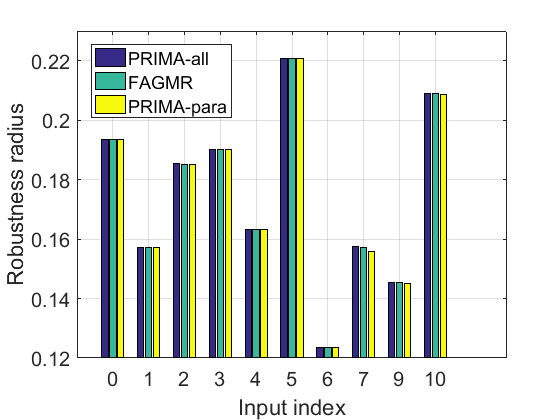
\includegraphics[width=0.7\textwidth]{figures/FigR3_2.png}
	\caption{Verified robustness radius by \prima-all, \prima-para, and \ourtool.} \label{table2}
	\end{center}
	%\vskip -0.1in
\end{figure}
%
%
%

%\vskip 0.1in

\subsection{Comparison with Other State-of-the-Art Verifiers}\label{Sec5.4}

We have shown \ourtool outperforms the state-of-the-art multi-neuron relaxation verifier \prima.
Besides this, it is necessary to know the performance position of \ourtool among other
kinds of state-of-the-art verifiers.
\begin{figure}  
\begin{center}
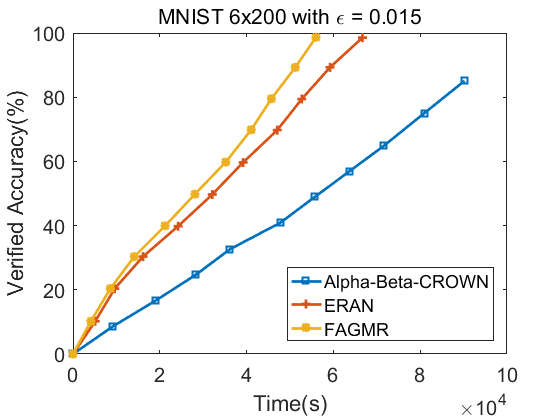
\includegraphics[width=5cm]{figures/state_6x200_0.015_mnist}
%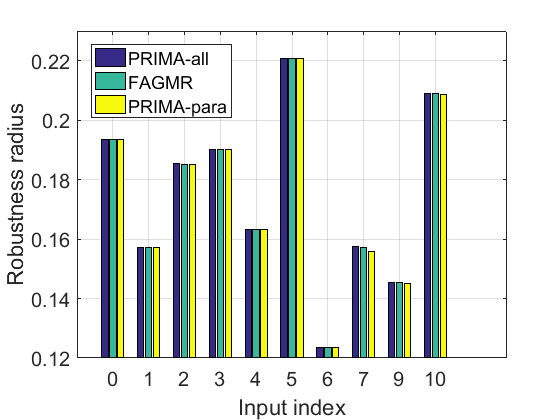
\includegraphics[width=4.7cm]{figures/FigR3_2.png}  
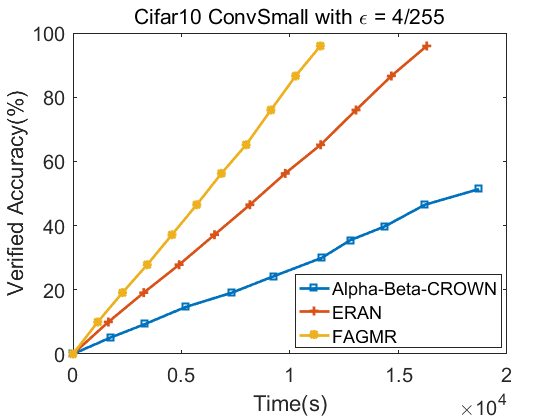
\includegraphics[width=5cm]{figures/state_convsmall_4255_cifar10.png}  
\caption{Comparisons on \mnist 6 $\times$ 200 with $\varepsilon=0.015$, 
%ConvBig(\mnist)
and ConvSmall(\cifar) with $\varepsilon=4/255$ respectively.}
\label{comparison}
\end{center}
%\vskip -0.1in
\end{figure}
Figure~\ref{comparison} shows the comparison of runtime and precision of \ourtool with other state-of-the-art verifiers, including \abcrown~\cite{DBLP:conf/iclr/XuZ0WJLH21} and \eran, which are both outstanding verifiers in VNN-COMP 2021~\cite{DBLP:journals/corr/abs-2109-00498}. \abcrown is an efficient verifier that uses symbol propagation methods~\cite{DBLP:conf/nips/ZhangWCHD18} represented as matrices, and its relaxation method is single-neuron based. \eran is also an efficient verification toolbox with several verifiers that rely on LP or MILP solvers, or symbolic propagation solvers, and one of its relaxation methods is \prima.

We use their default configurations and perform comparisons on the 6$\times$200 \mnist network and ConvSmall(\cifar). The results show that \abcrown has lower precision and longer runtime than both \eran and \ourtool. This can be attributed to \abcrown's use of single-neuron relations that lead to lower precision and the fact that it uses symbolic propagation with MILP and BaB strategy, which requires more iterations and runtime. 

Regarding the comparison between \eran and \ourtool, we observed that \ourtool runs 23.1\% faster than \eran on average with one more verified on the two benchmarks with small turbulences. Therefore, \ourtool can be considered as one of the competitive network verifiers.


%
%
%
\subsection{Comparison on Tanh and Sigmoid Neural Networks}\label{Sec5.5}
As mentioned in Section \ref{sec-generalization}, \ourtool can also be applied to other activations such
as Singmoid and Tanh. 
In this experiment, we compare the performance of \prima-para and \ourtool on the non-piecewise-linear activation functions, Tanh and Sigmoid, using the \mnist dataset. We evaluate 100 images on \mnist $6\times 500$(3000 neurons) and ConvMed(5704 neurons), both datasets can be obtained from the \eran homepage~\cite{ref_url4}. However, due to out-of-memory issues, \prima-all is excluded from this experiment.
\ourtool is configured similarly to \prima-para, except we have omitted parameters. In Table~\ref{table3}, we observe that \ourtool is 8.4\% faster than \prima-para on average with the same number of verified. These results demonstrate that \ourtool is a general method that performs better than the current state-of-the-art to some extent.

% \begin{table*}[htbp]
% \caption{Average groups number, average runtime, and verified number of \ourtool vs. \prima-para under perturbation threshold $\varepsilon$ on Sigmoid or Tanh networks}\label{table3}
% \vskip 0.01in
% %\resizebox{\linewidth}{!}{
% \centering
% \begin{small}
% %\setlength{\tabcolsep}{0.001mm}{
% \begin{tabular}[width=\linewidth]{c|c|c|c|c|c|c|c|c|c}
% \cline{1-10}
% \multicolumn{1}{c|}{Network} &\multicolumn{1}{|c|}{$Acc. $} &\multicolumn{1}{|c|}{$Activation $}&\multicolumn{1}{|c|}{$\varepsilon $}  & \multicolumn{3}{|c|}{\prima-para} &\multicolumn{3}{|c}{\ourtool}\\
% \cline{1-10}
% & &  & & groups  & time(\emph{s}) & veri. & groups & time(\emph{s}) & veri. \\
% \cline{1-10}
% \multirow{1}{*}{\makecell{MNIST \\ $6\times$500}}& 95 & Sigmoid& 0.012  & 6.2K & 640.9 & 95 & \textbf{3.8K} & \textbf{570.0} & \textbf{95}\\[2ex]

% %\hline

% %\multirow{1}{*}{\makecell{MNIST \\$9\times$100}} & 947 & 0.015 & - & - & - & 362.4K & 43.3K & 934 & \textbf{178.0K} & \textbf{41.7K} & \textbf{934}\\[2ex]
% \hline
% \multirow{1}{*}{\makecell{\mnist \\ConvMed}} & 99& Sigmoid & 0.014 & 6.3K & 255.6 & 99 & \textbf{5.9K} & \textbf{252.5} & \textbf{99}\\[2ex]


% \hline
% \multirow{1}{*}{\makecell{\mnist \\6$\times$500}} & 99 & Tanh & 0.005 & - & - & - &\textbf{184.8} & \textbf{194.9} & \textbf{98}\\[2ex]
% %\cline{3-12}
% % &  & 0.026 &  &  &  &  &  &  &  &  & \\

% %\hline
% %\multirow{1}{*}{\makecell{\mnist \\9$\times$200}} &  & 0.014 &  &  &  &  &  &  &  &  & \\[2ex]




% \hline
% \multirow{1}{*}{\makecell{\mnist \\ConvMed}} & 98& Tanh  & 0.005 & 1.2K & 220.4 & 98 & \textbf{446.3} & \textbf{191.8} & \textbf{98}\\[2ex]


% \hline


% \end{tabular}
% \end{small}
% %}}
% \vskip -0.01in
% \end{table*}


\begin{table*}[!t]
   \caption{Average groups number $g$, average runtime $t$(s), and verification precision $v$ 
            on Sigmoid or Tanh networks.}
   \label{table3}
   \centering
      \setlength{\tabcolsep}{0.5em}
      \resizebox{\textwidth}{!}{
      \small
      \begin{tabular}[width=\linewidth]{cccccccccc}
      \toprule[1pt]
      \multirow{2}*{Network} & \multirow{2}*{Total} & \multirow{2}*{Activation} & 
      \multirow{2}*{$\epsilon$} &
      \multicolumn{3}{c}{\prima-para} & \multicolumn{3}{c}{\ourtool}\\
   
      \cmidrule(lr){5-7} \cmidrule(lr){8-10}
      & & & & $g$ & $t$ & $v$ & $g$ & $t$ & $v$ \\
      \midrule[1pt]
   
      \makecell{\mnist \\ $6 \times 500$} & 95 & Sigmoid & 0.012  & 6.2K & 640.9 & 95 & 
      \textbf{3.8K} & \textbf{570.0} & 95 \\

      \midrule
      \makecell{\mnist \\ ConvMed} & 99 & Sigmoid & 0.014 & 6.3K & 255.6 & 99 & 
      \textbf{5.9K} & \textbf{252.5} & 99 \\

      \midrule
      \makecell{\mnist \\ 6$\times$500}& 99 & Tanh & 0.005 & - & - & - &
      \textbf{184.8} & \textbf{194.9} & \textbf{98} \\

      \midrule
      \makecell{\mnist \\ ConvMed} & 98 & Tanh  & 0.005 & 1.2K & 220.4 & 98 & 
      \textbf{446.3} & \textbf{191.8} & 98 \\

      \bottomrule[1pt]
      \end{tabular}}
      \end{table*}


\section{Related Work}\label{related work}

According to the completeness of the verification result, neural network verification
methods can be categorized into complete verification methods and incomplete methods.
% Incomplete verification methods often relax non-linear activations such as
% ReLU to speed up verification.
% Multi-neuron relaxation is one of the incomplete verification methods.

\paragraph{Complete Verification.}
Complete verification methods can describe the exact behavior
of a neural network on an input region. They can be further
classified into: (1)~SAT/SMT based
methods~\cite{DBLP:conf/cav/KatzBDJK17,DBLP:conf/cav/KatzHIJLLSTWZDK19,DBLP:conf/atva/Ehlers17},
which encodes the verification problem into an SAT/SMT query;
(2)~Mixed-integer linear programming (MILP) based
methods~\cite{DBLP:conf/atva/Ehlers17,DBLP:journals/mp/AndersonHMTV20,DBLP:conf/aaai/BotoevaKKLM20},
which encodes the verification into a MILP problem and is solved by specific solvers.
(3)~Branch-and-Bound based methods, which split non-linear
activation functions into linear
pieces~\cite{DBLP:conf/iclr/XuZ0WJLH21,DBLP:conf/nips/WangPWYJ18,DBLP:journals/jmlr/BunelLTTKK20,NEURIPS2021_fac7fead},
or split the input region to be small enough so that the neural
network behaves linearly on each input
sub-region~\cite{DBLP:conf/uss/WangPWYJ18}.
Complete methods are
limited in scalability because of the computational complexity.

\paragraph{Incomplete Verification.}
Incomplete verification methods often relax non-linear activations such as
ReLU to speed up verification.
Most incomplete methods attempt to develop efficient and precise
over-approximations for a given activation function
(e.g.~\cite{NEURIPS2018_f2f44698,DBLP:journals/pacmpl/SinghGPV19,DBLP:conf/nips/ZhangWCHD18,DBLP:conf/nips/SalmanY0HZ19,DBLP:conf/iclr/XuZ0WJLH21,Zheng2022},
see a survey in~\cite{DBLP:journals/ftopt/LiuALSBK21}).  
\ourtool belongs to this category. It applies convex relaxation 
to over-approximate non-linear
activation functions, hence incomplete but are much faster and more
scalable than complete methods.

\paragraph{Single-neuron Relaxation.}

Single-neuron
convex relaxation-based methods consider each neuron separately
and over-approximate its activation function.
They are efficient enough~\cite{NEURIPS2018_f2f44698,DBLP:journals/pacmpl/SinghGPV19,DBLP:conf/nips/ZhangWCHD18,DBLP:conf/nips/SalmanY0HZ19,DBLP:conf/iclr/XuZ0WJLH21,Zheng2022,zhao2022cleverest,goubault2021static},
but their verification precision is proved to be limited by a
convex relaxation barrier~\cite{DBLP:conf/nips/SalmanY0HZ19}.

\paragraph{Multi-neuron Relaxation.}
Multi-neuron convex relaxation
methods~\cite{DBLP:conf/nips/SinghGPV19,DBLP:conf/nips/TjandraatmadjaA20,DBLP:journals/pacmpl/MullerMSPV22}
suggest over-approximating jointly multiple neurons for higher
precision, hence breaking down the barrier faced by single-neuron
relaxation. Our work follows this promising direction and aims to
improve the efficiency of existing techniques.


%
%
%


\section{Conclusion}
\label{sec:conclusion}
In this paper, we propose an automatic, fast, and effective neuron grouping strategy for
multi-neuron convex relaxation methods.
Our key idea is computing the volume approximations of all possible $k$-neuron
groups and choose better ones for each neuron according to the computed volume.
The experiments show our strategy costs much less time and
has a precision advantage over the state-of-the-art tools.


%\subsubsection{Acknowledgements} Please place your acknowledgments at
%the end of the paper, preceded by an unnumbered run-in heading (i.e.
%3rd-level heading).

%
% ---- Bibliography ----
%
% BibTeX users should specify bibliography style 'splncs04'.
% References will then be sorted and formatted in the correct style.
%
\newpage
\bibliographystyle{splncs04}
\bibliography{references}


%

\end{document}
